\documentclass[tikz,border=0pt]{standalone}
\usepackage{xcolor}
\usetikzlibrary{calc}
% Palette: Sam_Comm_final.png by eye, each course's own, and data/frogs.json.
\definecolor{ink}{HTML}{3B2340}
\definecolor{sky}{HTML}{EFC46A}
\definecolor{skyhi}{HTML}{F5DA92}
\definecolor{skylow}{HTML}{E9B060}
\definecolor{cloud}{HTML}{F2D58A}
\definecolor{paper}{HTML}{FBEFD0}
\definecolor{cream}{HTML}{FFF6E0}
\definecolor{white}{HTML}{FFFFFF}
\definecolor{wallA}{HTML}{E88A73}
\definecolor{wallB}{HTML}{EE9F7E}
\definecolor{wallC}{HTML}{E47A7E}
\definecolor{wallD}{HTML}{F0B07E}
\definecolor{wallE}{HTML}{D9765F}
\definecolor{wallF}{HTML}{E99A8A}
\definecolor{greenA}{HTML}{8DBB7E}
\definecolor{greenB}{HTML}{6FA77A}
\definecolor{greenC}{HTML}{A9C97F}
\definecolor{greenD}{HTML}{5E9C6A}
\definecolor{greenE}{HTML}{4A8060}
\definecolor{meadow}{HTML}{B5CF86}
\definecolor{meadowdark}{HTML}{9DBE74}
\definecolor{window}{HTML}{F6E7A0}
\definecolor{windark}{HTML}{8C5A64}
\definecolor{metal}{HTML}{8D9A93}
\definecolor{metaldark}{HTML}{5E6B66}
\definecolor{wood}{HTML}{B9835A}
\definecolor{wooddark}{HTML}{8C5A3C}
\definecolor{woodlight}{HTML}{D9A66F}
\definecolor{rope}{HTML}{E3C48A}
\definecolor{stone}{HTML}{E7C9A0}
\definecolor{stonedark}{HTML}{C9A47E}
\definecolor{road}{HTML}{8E7A86}
\definecolor{roadline}{HTML}{F6E7A0}
\definecolor{kerb}{HTML}{D8B48C}
\definecolor{red}{HTML}{E0483E}
\definecolor{redlight}{HTML}{F27A6A}
\definecolor{gold}{HTML}{FFB000}
\definecolor{goldlight}{HTML}{FFD54F}
\definecolor{bell}{HTML}{F2B53A}
\definecolor{teal}{HTML}{4FA3A0}
\definecolor{tealdark}{HTML}{3C8582}
\definecolor{magenta}{HTML}{FF2E88}
\definecolor{cyan}{HTML}{13CFE3}
\definecolor{violet}{HTML}{8A5BD6}
\definecolor{water}{HTML}{6FB3A8}
\definecolor{waterlight}{HTML}{9FD3C6}
\definecolor{waterdark}{HTML}{4F8E86}
\definecolor{pad}{HTML}{7DB86A}
\definecolor{paddark}{HTML}{5C9A52}
\definecolor{padlight}{HTML}{A6D38A}
\definecolor{reed}{HTML}{8DB26A}
\definecolor{cattail}{HTML}{8A5A3C}
\definecolor{moss}{HTML}{A8B88E}
\definecolor{cypress}{HTML}{5E8A5A}
\definecolor{cypressdark}{HTML}{4A7048}
\definecolor{lotus}{HTML}{F48FB1}
\definecolor{lotusdark}{HTML}{E06C98}
\definecolor{lotuslight}{HTML}{FAD0DF}
\definecolor{lotuscentre}{HTML}{FFD54F}
\definecolor{lotusseed}{HTML}{E0A82E}
\definecolor{flybody}{HTML}{2B2530}
\definecolor{flyeye}{HTML}{E0242E}
\definecolor{flywing}{HTML}{F4F8FA}
\definecolor{mushred}{HTML}{E23B2E}
\definecolor{mushspot}{HTML}{FFF5E0}
\definecolor{stem}{HTML}{F2E2C2}
\definecolor{blush}{HTML}{F48FB1}
\definecolor{pupil}{HTML}{1A1220}
\definecolor{spider}{HTML}{3B2340}
\definecolor{swampskyhi}{HTML}{E9E3A0}
\definecolor{swampsky}{HTML}{D9D184}
\definecolor{swampskylow}{HTML}{C9C478}
\definecolor{swampcloud}{HTML}{EEE9B4}
\definecolor{swampwater}{HTML}{4F8A7F}
\definecolor{swampwaterlight}{HTML}{7AAE9C}
\definecolor{swampwaterdark}{HTML}{3F7268}
\definecolor{log}{HTML}{9A6A48}
\definecolor{logend}{HTML}{D9A66F}
\definecolor{dunehi}{HTML}{F7DFA0}
\definecolor{dunesky}{HTML}{F2C47A}
\definecolor{duneskylow}{HTML}{EBA865}
\definecolor{sand}{HTML}{EBC27C}
\definecolor{sandlight}{HTML}{F4D69C}
\definecolor{sanddark}{HTML}{D9A35E}
\definecolor{sanddeep}{HTML}{C98C4E}
\definecolor{sun}{HTML}{FFE6A3}
\definecolor{cactus}{HTML}{6FA77A}
\definecolor{cactusdark}{HTML}{4F8A60}
\definecolor{palmtrunk}{HTML}{B98A5A}
\definecolor{rock}{HTML}{C98C6A}
\definecolor{awning}{HTML}{4FA3A0}
\definecolor{carA}{HTML}{4FA3A0}
\definecolor{carB}{HTML}{F2B53A}
\definecolor{carC}{HTML}{E47A7E}
\definecolor{carD}{HTML}{8DBB7E}
\definecolor{glass}{HTML}{BFE3E0}
\definecolor{duskhi}{HTML}{6B4A6E}
\definecolor{dusk}{HTML}{B9607A}
\definecolor{dusklow}{HTML}{E9906A}
\definecolor{duskcloud}{HTML}{8E6680}
\definecolor{smoke}{HTML}{9C8494}
\definecolor{smokedark}{HTML}{7E6878}
\definecolor{basalt}{HTML}{4A3A4A}
\definecolor{basaltdark}{HTML}{352838}
\definecolor{basalttop}{HTML}{6E5868}
\definecolor{rockface}{HTML}{5E4A5C}
\definecolor{lava}{HTML}{FF6A1A}
\definecolor{lavagold}{HTML}{FFB000}
\definecolor{lavadark}{HTML}{C9481A}
\definecolor{pool}{HTML}{5FB8B0}
\definecolor{poollight}{HTML}{9FE0D6}
\definecolor{fungskyhi}{HTML}{C9B6E4}
\definecolor{fungsky}{HTML}{DAC7EC}
\definecolor{fungskylow}{HTML}{EBD9F2}
\definecolor{fungcloud}{HTML}{F5ECF9}
\definecolor{fungmoss}{HTML}{8FB97E}
\definecolor{fungmossdark}{HTML}{6F9E72}
\definecolor{fungmosslight}{HTML}{B2D199}
\definecolor{farbark}{HTML}{A58BAE}
\definecolor{bumper}{HTML}{4A8FE7}
\definecolor{bumperlight}{HTML}{8FC4FF}
\definecolor{bumperspot}{HTML}{E6F2FF}
\definecolor{gill}{HTML}{EADBC0}
\definecolor{shelf}{HTML}{E8B07A}
\definecolor{shelfdark}{HTML}{C98C4E}
\definecolor{glowteal}{HTML}{4FD6C4}
\definecolor{glowtealhi}{HTML}{A8F2E6}
\definecolor{glowviolet}{HTML}{A77FE8}
\definecolor{glowviolethi}{HTML}{D9C4FF}
\definecolor{puff}{HTML}{F3EAD8}
\definecolor{puffdark}{HTML}{D9C9A8}
\definecolor{cliff}{HTML}{9C8AA8}
\definecolor{cliffdark}{HTML}{7E6C8C}
\definecolor{foam}{HTML}{F4FBFA}
\definecolor{bubble}{HTML}{D4F6F8}
\definecolor{bubbleteal}{HTML}{7FE0D8}
\definecolor{bubbleviolet}{HTML}{C9A8F0}
\definecolor{bubblepink}{HTML}{F7B8D8}
\definecolor{crown}{HTML}{FFC23A}
\definecolor{crowndark}{HTML}{E09A1A}
\definecolor{jewel}{HTML}{E0483E}
\definecolor{jewelb}{HTML}{4FA3A0}
\definecolor{limeskin}{HTML}{7BC043}
\definecolor{limebelly}{HTML}{F4E8B0}
\definecolor{limemark}{HTML}{3C7DC4}
\definecolor{limeeye}{HTML}{E23B2E}
\definecolor{limefeet}{HTML}{F2913D}
\definecolor{azureskin}{HTML}{2E6FD8}
\definecolor{azurebelly}{HTML}{1F4FA0}
\definecolor{azuremark}{HTML}{16163A}
\definecolor{azureeye}{HTML}{16163A}
\definecolor{azurefeet}{HTML}{1F4FA0}
\definecolor{bumbleskin}{HTML}{232028}
\definecolor{bumblebelly}{HTML}{2E2A33}
\definecolor{bumblemark}{HTML}{F6CF2E}
\definecolor{bumbleeye}{HTML}{16163A}
\definecolor{bumblefeet}{HTML}{232028}
\definecolor{tomatoskin}{HTML}{E2522F}
\definecolor{tomatobelly}{HTML}{F6D9B8}
\definecolor{tomatomark}{HTML}{B83A22}
\definecolor{tomatoeye}{HTML}{3A2A1E}
\definecolor{tomatofeet}{HTML}{C9442A}
\definecolor{bufoskin}{HTML}{9A7A4E}
\definecolor{bufobelly}{HTML}{E8D6A8}
\definecolor{bufomark}{HTML}{6B5233}
\definecolor{bufoeye}{HTML}{E8B83A}
\definecolor{bufofeet}{HTML}{8A6C44}
\definecolor{goldieskin}{HTML}{F59A1B}
\definecolor{goldiebelly}{HTML}{F8C25A}
\definecolor{goldiemark}{HTML}{D97C0E}
\definecolor{goldieeye}{HTML}{2A1A10}
\definecolor{goldiefeet}{HTML}{E8890F}
\definecolor{chompskin}{HTML}{A7C957}
\definecolor{chompbelly}{HTML}{F2E6B8}
\definecolor{chompmark}{HTML}{6A4A2E}
\definecolor{chompeye}{HTML}{C9A227}
\definecolor{chompfeet}{HTML}{8DAF45}
\definecolor{glassyskin}{HTML}{B9E3C6}
\definecolor{glassybelly}{HTML}{E4F4EA}
\definecolor{glassymark}{HTML}{F2E25C}
\definecolor{glassyeye}{HTML}{E9E0C8}
\definecolor{glassyfeet}{HTML}{9FD3B0}
\newcommand{\Ink}{1.15pt}
\tikzset{inked/.style={draw=ink, line width=\Ink, line join=round, line cap=round}}
\begin{document}
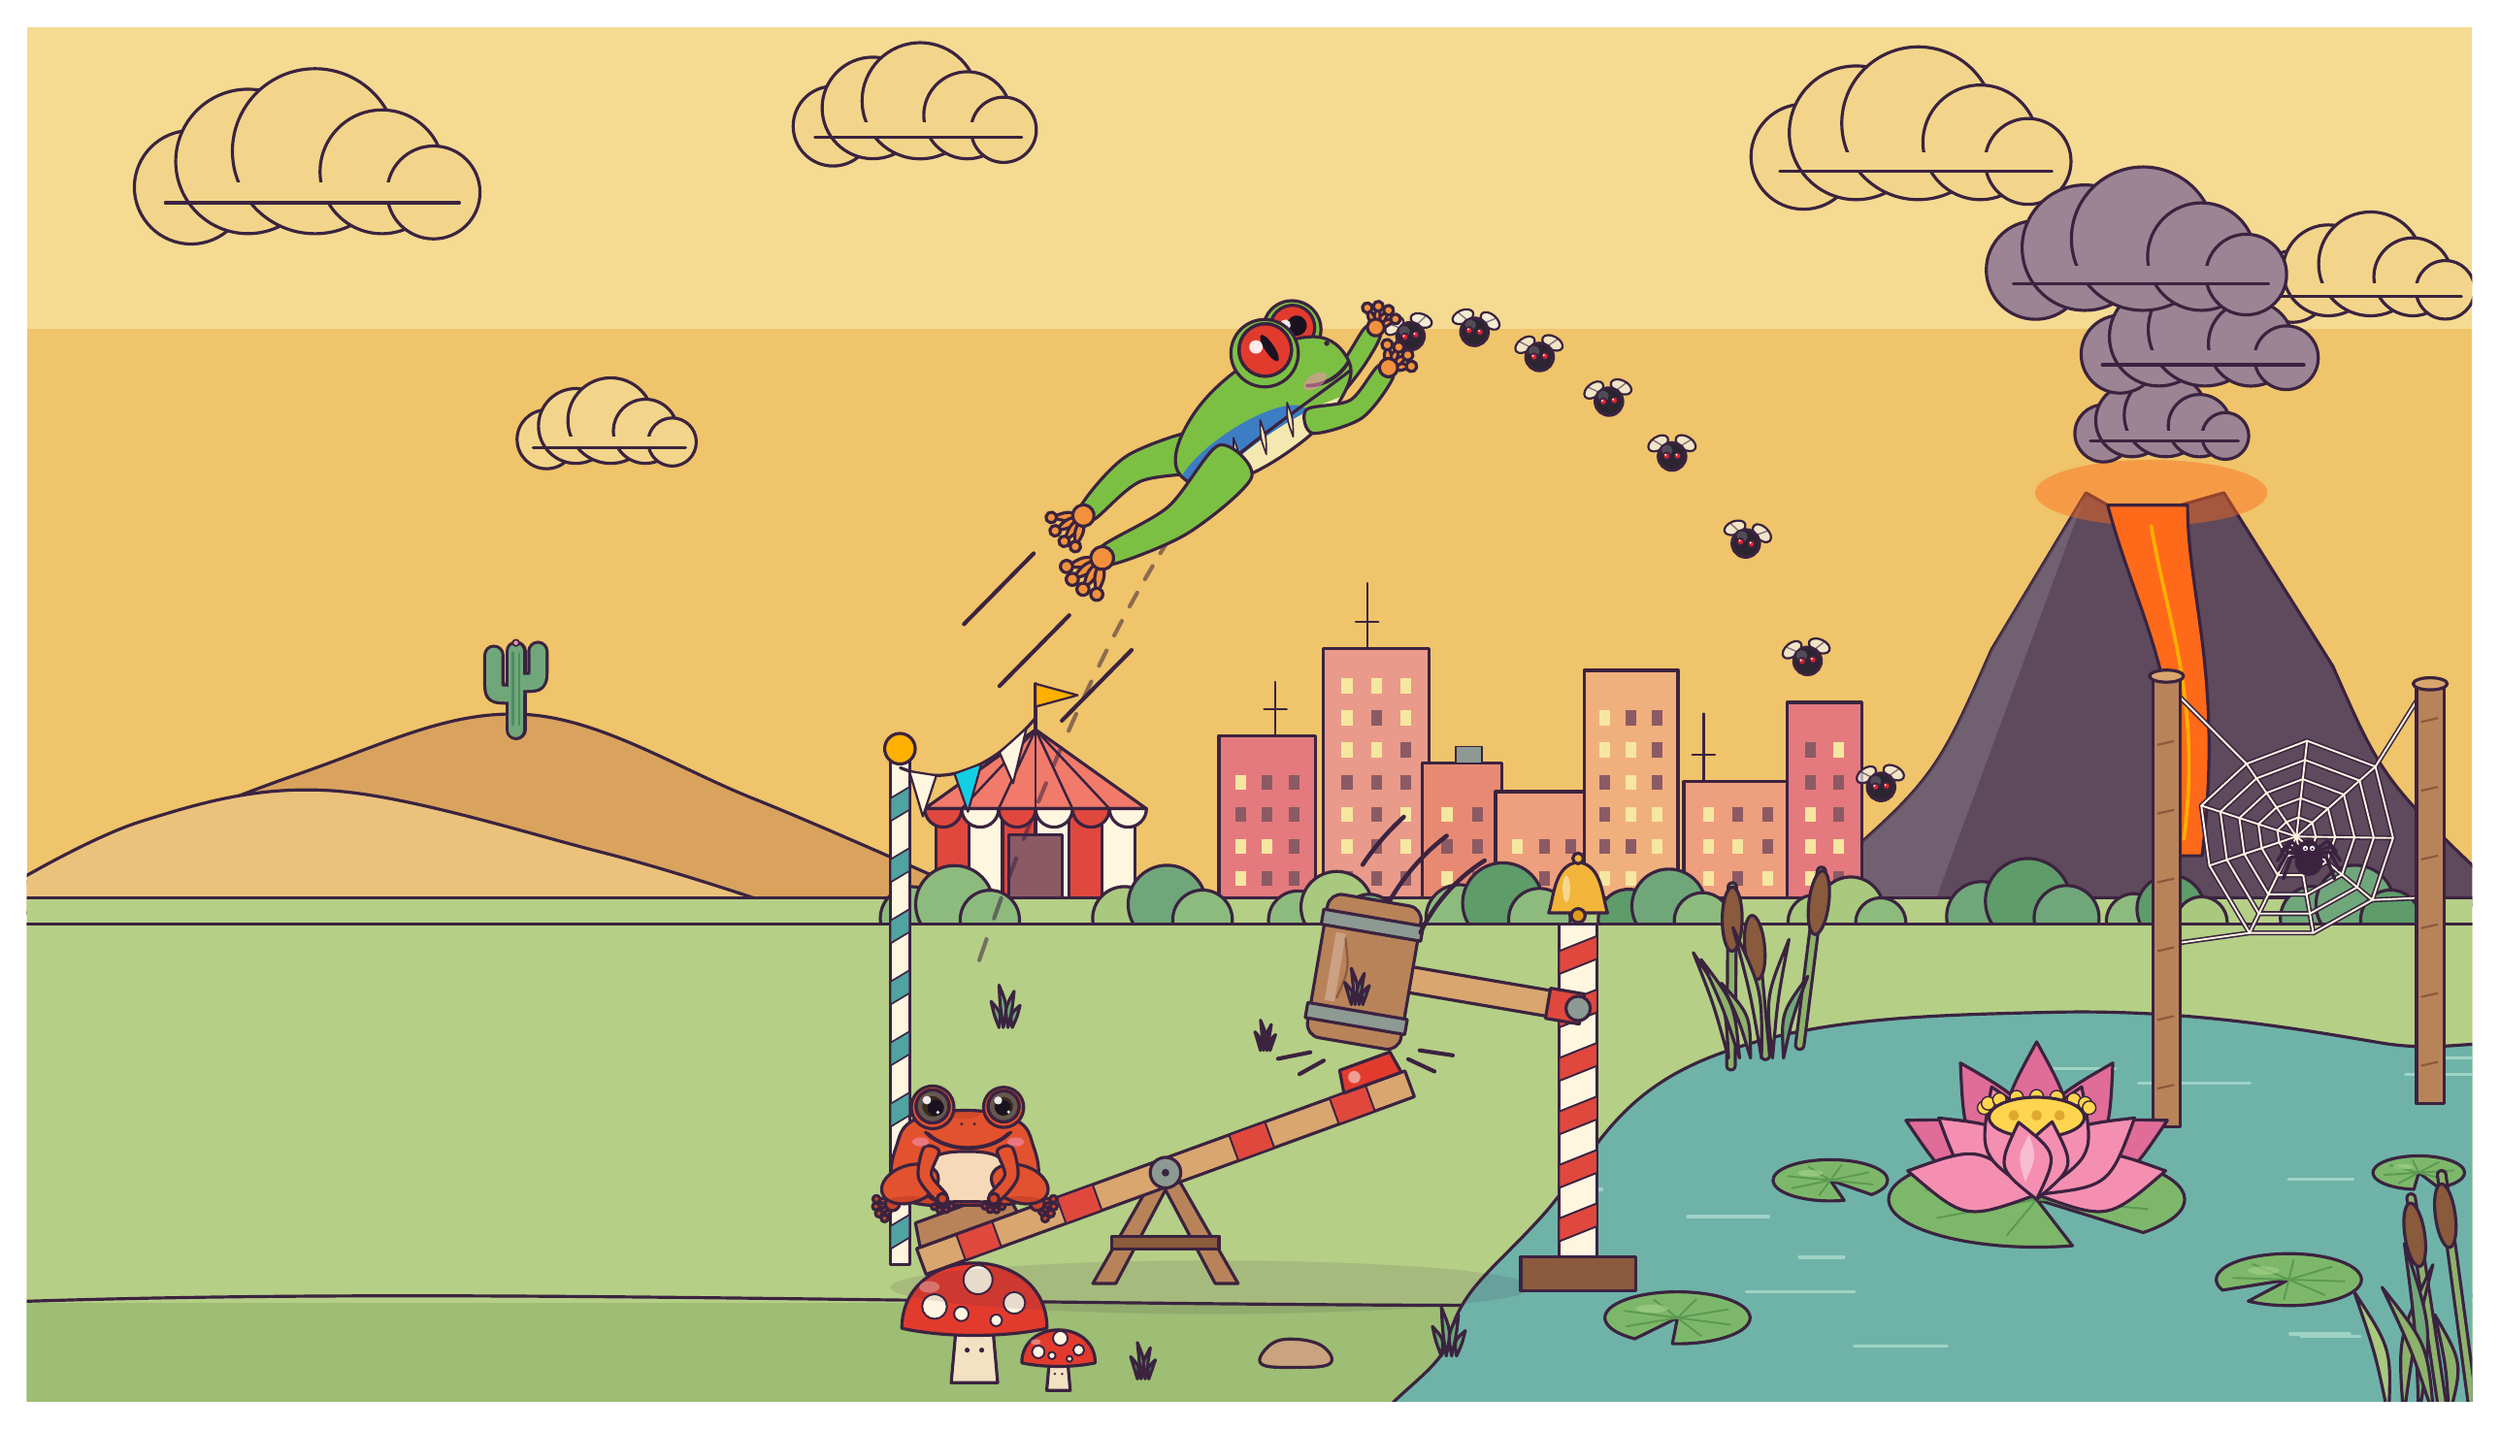
\begin{tikzpicture}
\clip (0,0) rectangle (32,18);
\fill[sky] (0,0) rectangle (32,18);
\fill[skyhi] (0,14.04) rectangle (32,18);
\fill[skylow] (0,0) rectangle (32,5.4);
\filldraw[inked,fill=cloud] (2.15,15.9) circle (0.743);
\filldraw[inked,fill=cloud] (2.893,16.238) circle (0.945);
\filldraw[inked,fill=cloud] (3.77,16.372) circle (1.08);
\filldraw[inked,fill=cloud] (4.647,16.102) circle (0.81);
\filldraw[inked,fill=cloud] (5.322,15.832) circle (0.608);
\fill[cloud] (2.15,15.697) rectangle (5.322,15.968);
\draw[ink, line width=1.15pt, line cap=round] (1.812,15.697) -- (5.66,15.697);
\filldraw[inked,fill=cloud] (10.55,16.7) circle (0.522);
\filldraw[inked,fill=cloud] (11.072,16.938) circle (0.665);
\filldraw[inked,fill=cloud] (11.69,17.032) circle (0.76);
\filldraw[inked,fill=cloud] (12.307,16.842) circle (0.57);
\filldraw[inked,fill=cloud] (12.783,16.652) circle (0.427);
\fill[cloud] (10.55,16.558) rectangle (12.783,16.747);
\draw[ink, line width=1.15pt, line cap=round] (10.312,16.558) -- (13.02,16.558);
\filldraw[inked,fill=cloud] (23.25,16.3) circle (0.688);
\filldraw[inked,fill=cloud] (23.938,16.613) circle (0.875);
\filldraw[inked,fill=cloud] (24.75,16.738) circle (1);
\filldraw[inked,fill=cloud] (25.562,16.488) circle (0.75);
\filldraw[inked,fill=cloud] (26.188,16.238) circle (0.562);
\fill[cloud] (23.25,16.113) rectangle (26.188,16.363);
\draw[ink, line width=1.15pt, line cap=round] (22.938,16.113) -- (26.5,16.113);
\filldraw[inked,fill=cloud] (29.65,14.6) circle (0.468);
\filldraw[inked,fill=cloud] (30.117,14.812) circle (0.595);
\filldraw[inked,fill=cloud] (30.67,14.897) circle (0.68);
\filldraw[inked,fill=cloud] (31.223,14.727) circle (0.51);
\filldraw[inked,fill=cloud] (31.648,14.557) circle (0.383);
\fill[cloud] (29.65,14.473) rectangle (31.648,14.643);
\draw[ink, line width=1.15pt, line cap=round] (29.438,14.473) -- (31.86,14.473);
\filldraw[inked,fill=cloud] (6.8,12.6) circle (0.385);
\filldraw[inked,fill=cloud] (7.185,12.775) circle (0.49);
\filldraw[inked,fill=cloud] (7.64,12.845) circle (0.56);
\filldraw[inked,fill=cloud] (8.095,12.705) circle (0.42);
\filldraw[inked,fill=cloud] (8.445,12.565) circle (0.315);
\fill[cloud] (6.8,12.495) rectangle (8.445,12.635);
\draw[ink, line width=1.15pt, line cap=round] (6.625,12.495) -- (8.62,12.495);
\filldraw[inked,fill=sanddark] plot[smooth, tension=0.6] coordinates {(-0.5,6.6) (3.5,8.2) (6.5,9) (9.5,7.9) (12.5,6.6)} -- (12.5,6.4) -- (-0.5,6.4) -- cycle;
\filldraw[inked,fill=sand] plot[smooth, tension=0.6] coordinates {(-0.5,6.6) (1.5,7.6) (4,8) (7.5,7.2) (9.5,6.6)} -- (9.5,6.4) -- (-0.5,6.4) -- cycle;
\draw[ink, line width=7.945pt, line cap=round, line join=round] plot[smooth, tension=0.4] coordinates {(6.4,8.8) (6.4,9.824)};
\draw[ink, line width=7.945pt, line cap=round, line join=round] plot[smooth, tension=0.4] coordinates {(6.4,9.261) (6.144,9.277) (6.112,9.389) (6.112,9.773)};
\draw[ink, line width=7.945pt, line cap=round, line join=round] plot[smooth, tension=0.4] coordinates {(6.4,9.414) (6.656,9.43) (6.688,9.542) (6.688,9.824)};
\draw[cactus, line width=5.645pt, line cap=round, line join=round] plot[smooth, tension=0.4] coordinates {(6.4,8.8) (6.4,9.824)};
\draw[cactus, line width=5.645pt, line cap=round, line join=round] plot[smooth, tension=0.4] coordinates {(6.4,9.261) (6.144,9.277) (6.112,9.389) (6.112,9.773)};
\draw[cactus, line width=5.645pt, line cap=round, line join=round] plot[smooth, tension=0.4] coordinates {(6.4,9.414) (6.656,9.43) (6.688,9.542) (6.688,9.824)};
\draw[cactusdark, line width=0.9pt, line cap=round] (6.362,8.864) -- (6.362,9.808);
\draw[cactusdark, line width=0.9pt, line cap=round] (6.442,8.864) -- (6.442,9.792);
\filldraw[inked,fill=lotus,line width=0.6pt] (6.4,9.936) circle (0.042);
\filldraw[inked,fill=rockface] (23.05,6.5) .. controls (24.95,8.12) .. (25.71,9.848) -- (26.945,11.9) -- (27.42,11.63) -- (28.18,11.738) -- (28.75,11.9) -- (30.175,9.632) .. controls (30.84,8.12) .. (32.55,6.5) -- cycle;
\fill[white, opacity=0.12] (26.945,11.9) -- (25.71,9.848) .. controls (24.95,8.12) .. (23.05,6.5) -- (24.95,6.5) -- cycle;
\fill[lava, opacity=0.45] (27.8,11.9) ellipse (1.52 and 0.432);
\filldraw[inked,fill=lava] (27.23,11.738) .. controls (27.61,10.28) and (28.37,9.2) .. (27.99,7.148) -- (28.465,7.148) .. controls (28.75,9.47) and (28.275,10.55) .. (28.275,11.738) -- cycle;
\draw[lavagold, line width=1.3pt, line cap=round] (27.8,11.468) .. controls (27.99,10.28) and (28.465,9.2) .. (28.227,7.364);
\filldraw[inked,fill=smoke] (27.174,12.678) circle (0.374);
\filldraw[inked,fill=smoke] (27.548,12.847) circle (0.475);
\filldraw[inked,fill=smoke] (27.989,12.915) circle (0.543);
\filldraw[inked,fill=smoke] (28.431,12.779) circle (0.408);
\filldraw[inked,fill=smoke] (28.77,12.644) circle (0.306);
\fill[smoke] (27.174,12.576) rectangle (28.77,12.712);
\draw[ink, line width=1.15pt, line cap=round] (27.004,12.576) -- (28.94,12.576);
\filldraw[inked,fill=smoke] (27.391,13.714) circle (0.509);
\filldraw[inked,fill=smoke] (27.9,13.946) circle (0.648);
\filldraw[inked,fill=smoke] (28.502,14.039) circle (0.741);
\filldraw[inked,fill=smoke] (29.104,13.853) circle (0.556);
\filldraw[inked,fill=smoke] (29.568,13.668) circle (0.417);
\fill[smoke] (27.391,13.575) rectangle (29.568,13.761);
\draw[ink, line width=1.15pt, line cap=round] (27.159,13.575) -- (29.799,13.575);
\filldraw[inked,fill=smoke] (26.286,14.816) circle (0.645);
\filldraw[inked,fill=smoke] (26.931,15.109) circle (0.821);
\filldraw[inked,fill=smoke] (27.694,15.227) circle (0.939);
\filldraw[inked,fill=smoke] (28.456,14.992) circle (0.704);
\filldraw[inked,fill=smoke] (29.043,14.757) circle (0.528);
\fill[smoke] (26.286,14.64) rectangle (29.043,14.875);
\draw[ink, line width=1.15pt, line cap=round] (25.993,14.64) -- (29.336,14.64);
\filldraw[inked,fill=wallC] (15.6,6.5) rectangle (16.868,8.715);
\fill[window] (15.812,6.75) rectangle (15.952,6.95);
\fill[window] (15.812,7.17) rectangle (15.952,7.37);
\fill[windark] (15.812,7.59) rectangle (15.952,7.79);
\fill[window] (15.812,8.01) rectangle (15.952,8.21);
\fill[windark] (16.164,6.75) rectangle (16.304,6.95);
\fill[window] (16.164,7.17) rectangle (16.304,7.37);
\fill[windark] (16.164,7.59) rectangle (16.304,7.79);
\fill[windark] (16.164,8.01) rectangle (16.304,8.21);
\fill[windark] (16.516,6.75) rectangle (16.656,6.95);
\fill[windark] (16.516,7.17) rectangle (16.656,7.37);
\fill[windark] (16.516,7.59) rectangle (16.656,7.79);
\fill[windark] (16.516,8.01) rectangle (16.656,8.21);
\draw[ink, line width=0.8pt, line cap=round] (16.337,8.715) -- (16.337,9.425);
\draw[ink, line width=0.7pt, line cap=round] (16.187,9.065) -- (16.487,9.065);
\filldraw[inked,fill=wallF] (16.963,6.5) rectangle (18.354,9.865);
\fill[windark] (17.206,6.75) rectangle (17.346,6.95);
\fill[window] (17.206,7.17) rectangle (17.346,7.37);
\fill[window] (17.206,7.59) rectangle (17.346,7.79);
\fill[windark] (17.206,8.01) rectangle (17.346,8.21);
\fill[window] (17.206,8.43) rectangle (17.346,8.63);
\fill[window] (17.206,8.85) rectangle (17.346,9.05);
\fill[window] (17.206,9.27) rectangle (17.346,9.47);
\fill[windark] (17.589,6.75) rectangle (17.729,6.95);
\fill[windark] (17.589,7.17) rectangle (17.729,7.37);
\fill[windark] (17.589,7.59) rectangle (17.729,7.79);
\fill[windark] (17.589,8.01) rectangle (17.729,8.21);
\fill[window] (17.589,8.43) rectangle (17.729,8.63);
\fill[windark] (17.589,8.85) rectangle (17.729,9.05);
\fill[window] (17.589,9.27) rectangle (17.729,9.47);
\fill[windark] (17.971,6.75) rectangle (18.111,6.95);
\fill[window] (17.971,7.17) rectangle (18.111,7.37);
\fill[window] (17.971,7.59) rectangle (18.111,7.79);
\fill[windark] (17.971,8.01) rectangle (18.111,8.21);
\fill[windark] (17.971,8.43) rectangle (18.111,8.63);
\fill[window] (17.971,8.85) rectangle (18.111,9.05);
\fill[window] (17.971,9.27) rectangle (18.111,9.47);
\draw[ink, line width=0.8pt, line cap=round] (17.538,9.865) -- (17.538,10.718);
\draw[ink, line width=0.7pt, line cap=round] (17.388,10.215) -- (17.688,10.215);
\filldraw[inked,fill=wallA] (18.261,6.5) rectangle (19.301,8.359);
\fill[window] (18.514,6.75) rectangle (18.654,6.95);
\fill[windark] (18.514,7.17) rectangle (18.654,7.37);
\fill[window] (18.514,7.59) rectangle (18.654,7.79);
\fill[windark] (18.908,6.75) rectangle (19.048,6.95);
\fill[windark] (18.908,7.17) rectangle (19.048,7.37);
\fill[windark] (18.908,7.59) rectangle (19.048,7.79);
\filldraw[inked,fill=metal,line width=0.7pt] (18.697,8.359) rectangle (19.047,8.579);
\filldraw[inked,fill=wallB] (19.218,6.5) rectangle (20.492,7.987);
\fill[windark] (19.432,6.75) rectangle (19.572,6.95);
\fill[window] (19.432,7.17) rectangle (19.572,7.37);
\fill[windark] (19.785,6.75) rectangle (19.925,6.95);
\fill[windark] (19.785,7.17) rectangle (19.925,7.37);
\fill[windark] (20.139,6.75) rectangle (20.279,6.95);
\fill[windark] (20.139,7.17) rectangle (20.279,7.37);
\filldraw[inked,fill=wallD] (20.376,6.5) rectangle (21.607,9.576);
\fill[window] (20.578,6.75) rectangle (20.718,6.95);
\fill[windark] (20.578,7.17) rectangle (20.718,7.37);
\fill[windark] (20.578,7.59) rectangle (20.718,7.79);
\fill[windark] (20.578,8.01) rectangle (20.718,8.21);
\fill[window] (20.578,8.43) rectangle (20.718,8.63);
\fill[window] (20.578,8.85) rectangle (20.718,9.05);
\fill[window] (20.921,6.75) rectangle (21.061,6.95);
\fill[windark] (20.921,7.17) rectangle (21.061,7.37);
\fill[window] (20.921,7.59) rectangle (21.061,7.79);
\fill[window] (20.921,8.01) rectangle (21.061,8.21);
\fill[window] (20.921,8.43) rectangle (21.061,8.63);
\fill[windark] (20.921,8.85) rectangle (21.061,9.05);
\fill[windark] (21.264,6.75) rectangle (21.404,6.95);
\fill[window] (21.264,7.17) rectangle (21.404,7.37);
\fill[window] (21.264,7.59) rectangle (21.404,7.79);
\fill[windark] (21.264,8.01) rectangle (21.404,8.21);
\fill[windark] (21.264,8.43) rectangle (21.404,8.63);
\fill[windark] (21.264,8.85) rectangle (21.404,9.05);
\filldraw[inked,fill=wallB] (21.682,6.5) rectangle (23.096,8.117);
\fill[window] (21.931,6.75) rectangle (22.071,6.95);
\fill[window] (21.931,7.17) rectangle (22.071,7.37);
\fill[window] (21.931,7.59) rectangle (22.071,7.79);
\fill[windark] (22.319,6.75) rectangle (22.459,6.95);
\fill[window] (22.319,7.17) rectangle (22.459,7.37);
\fill[windark] (22.319,7.59) rectangle (22.459,7.79);
\fill[window] (22.707,6.75) rectangle (22.847,6.95);
\fill[windark] (22.707,7.17) rectangle (22.847,7.37);
\fill[windark] (22.707,7.59) rectangle (22.847,7.79);
\draw[ink, line width=0.8pt, line cap=round] (21.942,8.117) -- (21.942,9.01);
\draw[ink, line width=0.7pt, line cap=round] (21.792,8.467) -- (22.092,8.467);
\filldraw[inked,fill=wallC] (23.038,6.5) rectangle (24.011,9.156);
\fill[window] (23.269,6.75) rectangle (23.409,6.95);
\fill[window] (23.269,7.17) rectangle (23.409,7.37);
\fill[window] (23.269,7.59) rectangle (23.409,7.79);
\fill[windark] (23.269,8.01) rectangle (23.409,8.21);
\fill[windark] (23.269,8.43) rectangle (23.409,8.63);
\fill[windark] (23.64,6.75) rectangle (23.78,6.95);
\fill[window] (23.64,7.17) rectangle (23.78,7.37);
\fill[windark] (23.64,7.59) rectangle (23.78,7.79);
\fill[windark] (23.64,8.01) rectangle (23.78,8.21);
\fill[window] (23.64,8.43) rectangle (23.78,8.63);
\filldraw[inked,fill=red] (11.9,6.5) -- (12.333,6.5) -- (12.333,7.765) -- (11.9,7.765) -- cycle;
\filldraw[inked,fill=cream] (12.333,6.5) -- (12.767,6.5) -- (12.767,7.765) -- (12.333,7.765) -- cycle;
\filldraw[inked,fill=red] (12.767,6.5) -- (13.2,6.5) -- (13.2,7.765) -- (12.767,7.765) -- cycle;
\filldraw[inked,fill=cream] (13.2,6.5) -- (13.633,6.5) -- (13.633,7.765) -- (13.2,7.765) -- cycle;
\filldraw[inked,fill=red] (13.633,6.5) -- (14.067,6.5) -- (14.067,7.765) -- (13.633,7.765) -- cycle;
\filldraw[inked,fill=cream] (14.067,6.5) -- (14.5,6.5) -- (14.5,7.765) -- (14.067,7.765) -- cycle;
\filldraw[inked,fill=redlight] (11.75,7.765) -- (14.65,7.765) -- (13.2,8.8) -- cycle;
\draw[ink, line width=0.9pt, line cap=round] (12.233,7.765) -- (13.2,8.8);
\draw[ink, line width=0.9pt, line cap=round] (12.717,7.765) -- (13.2,8.8);
\draw[ink, line width=0.9pt, line cap=round] (13.2,7.765) -- (13.2,8.8);
\draw[ink, line width=0.9pt, line cap=round] (13.683,7.765) -- (13.2,8.8);
\draw[ink, line width=0.9pt, line cap=round] (14.167,7.765) -- (13.2,8.8);
\filldraw[inked,fill=red] (11.75,7.765) arc[start angle=180, end angle=360, radius=0.242] -- cycle;
\filldraw[inked,fill=cream] (12.233,7.765) arc[start angle=180, end angle=360, radius=0.242] -- cycle;
\filldraw[inked,fill=red] (12.717,7.765) arc[start angle=180, end angle=360, radius=0.242] -- cycle;
\filldraw[inked,fill=cream] (13.2,7.765) arc[start angle=180, end angle=360, radius=0.242] -- cycle;
\filldraw[inked,fill=red] (13.683,7.765) arc[start angle=180, end angle=360, radius=0.242] -- cycle;
\filldraw[inked,fill=cream] (14.167,7.765) arc[start angle=180, end angle=360, radius=0.242] -- cycle;
\filldraw[inked,fill=windark] (12.85,6.5) -- (13.55,6.5) -- (13.55,7.42) -- (12.85,7.42) -- cycle;
\draw[ink, line width=1.2pt, line cap=round] (13.2,8.8) -- (13.2,9.4);
\filldraw[inked,fill=gold,line width=0.8pt] (13.2,9.4) -- (13.75,9.25) -- (13.2,9.1) -- cycle;
\filldraw[inked,fill=meadow] (-0.5,-0.5) rectangle (32.5,6.6);
\filldraw[inked,fill=greenA] (11.584,6.327) circle (0.416);
\filldraw[inked,fill=greenA] (12.139,6.512) circle (0.508);
\filldraw[inked,fill=greenA] (12.601,6.309) circle (0.388);
\filldraw[inked,fill=greenC] (14.364,6.328) circle (0.417);
\filldraw[inked,fill=greenB] (14.921,6.514) circle (0.51);
\filldraw[inked,fill=greenA] (15.385,6.31) circle (0.39);
\filldraw[inked,fill=greenA] (16.631,6.305) circle (0.383);
\filldraw[inked,fill=greenC] (17.141,6.475) circle (0.468);
\filldraw[inked,fill=greenB] (17.566,6.288) circle (0.357);
\filldraw[inked,fill=greenA] (18.74,6.338) circle (0.431);
\filldraw[inked,fill=greenD] (19.315,6.529) circle (0.527);
\filldraw[inked,fill=greenA] (19.794,6.318) circle (0.403);
\filldraw[inked,fill=greenD] (20.959,6.314) circle (0.396);
\filldraw[inked,fill=greenB] (21.487,6.49) circle (0.484);
\filldraw[inked,fill=greenA] (21.927,6.296) circle (0.369);
\filldraw[inked,fill=greenC] (23.399,6.285) circle (0.352);
\filldraw[inked,fill=greenC] (23.868,6.441) circle (0.43);
\filldraw[inked,fill=greenA] (24.26,6.269) circle (0.329);
\filldraw[inked,fill=greenB] (25.578,6.354) circle (0.456);
\filldraw[inked,fill=greenD] (26.186,6.556) circle (0.557);
\filldraw[inked,fill=greenB] (26.692,6.334) circle (0.425);
\filldraw[inked,fill=greenA] (27.573,6.291) circle (0.361);
\filldraw[inked,fill=greenD] (28.055,6.452) circle (0.442);
\filldraw[inked,fill=greenC] (28.457,6.275) circle (0.337);
\filldraw[inked,fill=greenB] (29.908,6.329) circle (0.418);
\filldraw[inked,fill=greenB] (30.466,6.514) circle (0.511);
\filldraw[inked,fill=greenD] (30.93,6.31) circle (0.39);
\filldraw[inked,fill=meadow] (-0.5,-0.5) rectangle (32.5,6.25);
\draw[ink, line width=1.15pt] (-0.5,6.25) -- (32.5,6.25);
\fill[meadowdark] (-0.5,-0.5) rectangle (32.5,1.3);
\draw[ink, line width=1.15pt] (-0.5,1.3) .. controls (8,1.6) and (16,1.0) .. (32.5,1.4);
\filldraw[inked,fill=water] plot[smooth cycle, tension=0.7] coordinates {(19.8,2.4) (22,4.5) (26.5,5.1) (30.8,4.7) (33,4) (33,-1) (19,-1) (18.6,0.8)};
\begin{scope}\clip plot[smooth cycle, tension=0.7] coordinates {(19.8,2.4) (22,4.5) (26.5,5.1) (30.8,4.7) (33,4) (33,-1) (19,-1) (18.6,0.8)};
\draw[waterlight, line width=1.3pt, line cap=round] (31.128,4.284) -- (32.011,4.284);
\draw[waterlight, line width=1.3pt, line cap=round] (31.463,4.503) -- (32.944,4.503);
\draw[waterlight, line width=1.3pt, line cap=round] (26.192,4.364) -- (27.33,4.364);
\draw[waterlight, line width=1.3pt, line cap=round] (23.915,0.729) -- (25.124,0.729);
\draw[waterlight, line width=1.3pt, line cap=round] (27.633,4.172) -- (29.092,4.172);
\draw[waterlight, line width=1.3pt, line cap=round] (19.912,2.783) -- (20.607,2.783);
\draw[waterlight, line width=1.3pt, line cap=round] (21.735,2.427) -- (22.792,2.427);
\draw[waterlight, line width=1.3pt, line cap=round] (29.306,1.292) -- (29.906,1.292);
\draw[waterlight, line width=1.3pt, line cap=round] (29.757,0.858) -- (30.534,0.858);
\draw[waterlight, line width=1.3pt, line cap=round] (29.62,0.889) -- (30.393,0.889);
\draw[waterlight, line width=1.3pt, line cap=round] (22.502,1.441) -- (23.916,1.441);
\draw[waterlight, line width=1.3pt, line cap=round] (23.197,1.896) -- (23.774,1.896);
\draw[waterlight, line width=1.3pt, line cap=round] (29.596,2.915) -- (30.439,2.915);
\draw[waterlight, line width=1.3pt, line cap=round] (26.481,2.967) -- (27.354,2.967);
\end{scope}
\draw[ink, line width=1.84pt, line cap=round, line join=round] (29.7,7.4) -- (30.964,7.381);
\draw[ink, line width=1.84pt, line cap=round, line join=round] (29.7,7.4) -- (30.733,8.316);
\draw[ink, line width=1.84pt, line cap=round, line join=round] (29.7,7.4) -- (29.839,8.654);
\draw[ink, line width=1.84pt, line cap=round, line join=round] (29.7,7.4) -- (29.046,8.352);
\draw[ink, line width=1.84pt, line cap=round, line join=round] (29.7,7.4) -- (28.455,7.805);
\draw[ink, line width=1.84pt, line cap=round, line join=round] (29.7,7.4) -- (28.561,7.02);
\draw[ink, line width=1.84pt, line cap=round, line join=round] (29.7,7.4) -- (29.086,6.139);
\draw[ink, line width=1.84pt, line cap=round, line join=round] (29.7,7.4) -- (29.92,6.138);
\draw[ink, line width=1.84pt, line cap=round, line join=round] (29.7,7.4) -- (30.693,6.57);
\draw[ink, line width=1.84pt, line cap=round, line join=round] (29.953,7.396) -- (29.907,7.583) -- (29.728,7.651) -- (29.569,7.59) -- (29.451,7.481) -- (29.472,7.324) -- (29.577,7.148) -- (29.744,7.148) -- (29.899,7.234) -- (29.953,7.396);
\draw[ink, line width=1.84pt, line cap=round, line join=round] (30.206,7.392) -- (30.113,7.767) -- (29.756,7.902) -- (29.438,7.781) -- (29.202,7.562) -- (29.245,7.248) -- (29.454,6.895) -- (29.788,6.895) -- (30.097,7.068) -- (30.206,7.392);
\draw[ink, line width=1.84pt, line cap=round, line join=round] (30.459,7.389) -- (30.32,7.95) -- (29.783,8.152) -- (29.308,7.971) -- (28.953,7.643) -- (29.017,7.172) -- (29.332,6.643) -- (29.832,6.643) -- (30.296,6.902) -- (30.459,7.389);
\draw[ink, line width=1.84pt, line cap=round, line join=round] (30.712,7.385) -- (30.526,8.133) -- (29.811,8.403) -- (29.177,8.161) -- (28.704,7.724) -- (28.789,7.096) -- (29.209,6.391) -- (29.876,6.391) -- (30.494,6.736) -- (30.712,7.385);
\draw[ink, line width=1.84pt, line cap=round, line join=round] (30.964,7.381) -- (30.733,8.316) -- (29.839,8.654) -- (29.046,8.352) -- (28.455,7.805) -- (28.561,7.02) -- (29.086,6.139) -- (29.92,6.138) -- (30.693,6.57) -- (30.964,7.381);
\draw[ink, line width=1.84pt, line cap=round, line join=round] (29.046,8.352) -- (28.1,9.3);
\draw[ink, line width=1.84pt, line cap=round, line join=round] (30.733,8.316) -- (31.35,9.3);
\draw[ink, line width=1.84pt, line cap=round, line join=round] (29.086,6.139) -- (28.1,6);
\draw[ink, line width=1.84pt, line cap=round, line join=round] (30.693,6.57) -- (31.35,6.6);
\draw[cream, line width=0.69pt, line cap=round, line join=round] (29.7,7.4) -- (30.964,7.381);
\draw[cream, line width=0.69pt, line cap=round, line join=round] (29.7,7.4) -- (30.733,8.316);
\draw[cream, line width=0.69pt, line cap=round, line join=round] (29.7,7.4) -- (29.839,8.654);
\draw[cream, line width=0.69pt, line cap=round, line join=round] (29.7,7.4) -- (29.046,8.352);
\draw[cream, line width=0.69pt, line cap=round, line join=round] (29.7,7.4) -- (28.455,7.805);
\draw[cream, line width=0.69pt, line cap=round, line join=round] (29.7,7.4) -- (28.561,7.02);
\draw[cream, line width=0.69pt, line cap=round, line join=round] (29.7,7.4) -- (29.086,6.139);
\draw[cream, line width=0.69pt, line cap=round, line join=round] (29.7,7.4) -- (29.92,6.138);
\draw[cream, line width=0.69pt, line cap=round, line join=round] (29.7,7.4) -- (30.693,6.57);
\draw[cream, line width=0.69pt, line cap=round, line join=round] (29.953,7.396) -- (29.907,7.583) -- (29.728,7.651) -- (29.569,7.59) -- (29.451,7.481) -- (29.472,7.324) -- (29.577,7.148) -- (29.744,7.148) -- (29.899,7.234) -- (29.953,7.396);
\draw[cream, line width=0.69pt, line cap=round, line join=round] (30.206,7.392) -- (30.113,7.767) -- (29.756,7.902) -- (29.438,7.781) -- (29.202,7.562) -- (29.245,7.248) -- (29.454,6.895) -- (29.788,6.895) -- (30.097,7.068) -- (30.206,7.392);
\draw[cream, line width=0.69pt, line cap=round, line join=round] (30.459,7.389) -- (30.32,7.95) -- (29.783,8.152) -- (29.308,7.971) -- (28.953,7.643) -- (29.017,7.172) -- (29.332,6.643) -- (29.832,6.643) -- (30.296,6.902) -- (30.459,7.389);
\draw[cream, line width=0.69pt, line cap=round, line join=round] (30.712,7.385) -- (30.526,8.133) -- (29.811,8.403) -- (29.177,8.161) -- (28.704,7.724) -- (28.789,7.096) -- (29.209,6.391) -- (29.876,6.391) -- (30.494,6.736) -- (30.712,7.385);
\draw[cream, line width=0.69pt, line cap=round, line join=round] (30.964,7.381) -- (30.733,8.316) -- (29.839,8.654) -- (29.046,8.352) -- (28.455,7.805) -- (28.561,7.02) -- (29.086,6.139) -- (29.92,6.138) -- (30.693,6.57) -- (30.964,7.381);
\draw[cream, line width=0.69pt, line cap=round, line join=round] (29.046,8.352) -- (28.1,9.3);
\draw[cream, line width=0.69pt, line cap=round, line join=round] (30.733,8.316) -- (31.35,9.3);
\draw[cream, line width=0.69pt, line cap=round, line join=round] (29.086,6.139) -- (28.1,6);
\draw[cream, line width=0.69pt, line cap=round, line join=round] (30.693,6.57) -- (31.35,6.6);
\draw[ink, line width=1.265pt, line cap=round, line join=round] (29.862,7.157) -- (29.618,7.343) -- (29.502,7.202);
\draw[ink, line width=1.265pt, line cap=round, line join=round] (29.862,7.157) -- (29.583,7.273) -- (29.45,7.084);
\draw[ink, line width=1.265pt, line cap=round, line join=round] (29.862,7.157) -- (29.588,7.199) -- (29.459,6.959);
\draw[ink, line width=1.265pt, line cap=round, line join=round] (29.862,7.157) -- (29.634,7.133) -- (29.526,6.846);
\draw[ink, line width=1.265pt, line cap=round, line join=round] (29.862,7.157) -- (30.106,7.343) -- (30.222,7.202);
\draw[ink, line width=1.265pt, line cap=round, line join=round] (29.862,7.157) -- (30.141,7.273) -- (30.274,7.084);
\draw[ink, line width=1.265pt, line cap=round, line join=round] (29.862,7.157) -- (30.136,7.199) -- (30.265,6.959);
\draw[ink, line width=1.265pt, line cap=round, line join=round] (29.862,7.157) -- (30.09,7.133) -- (30.198,6.846);
\filldraw[inked,fill=spider] (29.862,7.068) circle (0.163);
\filldraw[inked,fill=spider] (29.862,7.231) circle (0.111);
\fill[white] (29.817,7.246) circle (0.033);
\fill[ink] (29.817,7.239) circle (0.015);
\fill[white] (29.907,7.246) circle (0.033);
\fill[ink] (29.907,7.239) circle (0.015);
\filldraw[inked,fill=wood] (27.82,3.6) rectangle (28.18,9.5);
\draw[wooddark, line width=0.8pt] (27.88,4.1) -- (28.1,4.15);
\draw[wooddark, line width=0.8pt] (27.88,5) -- (28.1,5.05);
\draw[wooddark, line width=0.8pt] (27.88,5.9) -- (28.1,5.95);
\draw[wooddark, line width=0.8pt] (27.88,6.8) -- (28.1,6.85);
\draw[wooddark, line width=0.8pt] (27.88,7.7) -- (28.1,7.75);
\draw[wooddark, line width=0.8pt] (27.88,8.6) -- (28.1,8.65);
\filldraw[inked,fill=woodlight] (28,9.5) ellipse (0.223 and 0.079);
\filldraw[inked,fill=wood] (31.27,3.9) rectangle (31.63,9.4);
\draw[wooddark, line width=0.8pt] (31.33,4.4) -- (31.55,4.45);
\draw[wooddark, line width=0.8pt] (31.33,5.3) -- (31.55,5.35);
\draw[wooddark, line width=0.8pt] (31.33,6.2) -- (31.55,6.25);
\draw[wooddark, line width=0.8pt] (31.33,7.1) -- (31.55,7.15);
\draw[wooddark, line width=0.8pt] (31.33,8) -- (31.55,8.05);
\draw[wooddark, line width=0.8pt] (31.33,8.9) -- (31.55,8.95);
\filldraw[inked,fill=woodlight] (31.45,9.4) ellipse (0.223 and 0.079);
\filldraw[inked,fill=pad] (21.6,1.1) -- ($(21.6,1.1)+(266:0.95 and 0.34)$) arc[start angle=266, end angle=594, x radius=0.95, y radius=0.34] -- cycle;
\draw[paddark, line width=0.7pt] (21.6,1.1) -- (21.913,0.86);
\draw[paddark, line width=0.7pt] (21.6,1.1) -- (22.296,1.009);
\draw[paddark, line width=0.7pt] (21.6,1.1) -- (22.272,1.212);
\draw[paddark, line width=0.7pt] (21.6,1.1) -- (21.853,1.349);
\draw[paddark, line width=0.7pt] (21.6,1.1) -- (21.287,1.34);
\draw[paddark, line width=0.7pt] (21.6,1.1) -- (20.904,1.191);
\draw[paddark, line width=0.7pt] (21.6,1.1) -- (20.928,0.988);
\fill[padlight, opacity=0.6] (21.268,1.219) ellipse (0.209 and 0.054);
\filldraw[inked,fill=pad] (23.6,2.9) -- ($(23.6,2.9)+(316:0.75 and 0.27)$) arc[start angle=316, end angle=644, x radius=0.75, y radius=0.27] -- cycle;
\draw[paddark, line width=0.7pt] (23.6,2.9) -- (24.165,2.845);
\draw[paddark, line width=0.7pt] (23.6,2.9) -- (24.107,3.005);
\draw[paddark, line width=0.7pt] (23.6,2.9) -- (23.751,3.103);
\draw[paddark, line width=0.7pt] (23.6,2.9) -- (23.308,3.082);
\draw[paddark, line width=0.7pt] (23.6,2.9) -- (23.035,2.955);
\draw[paddark, line width=0.7pt] (23.6,2.9) -- (23.093,2.795);
\draw[paddark, line width=0.7pt] (23.6,2.9) -- (23.449,2.697);
\fill[padlight, opacity=0.6] (23.338,2.994) ellipse (0.165 and 0.043);
\filldraw[inked,fill=pad] (29.6,1.6) -- ($(29.6,1.6)+(236:0.95 and 0.34)$) arc[start angle=236, end angle=564, x radius=0.95, y radius=0.34] -- cycle;
\draw[paddark, line width=0.7pt] (29.6,1.6) -- (29.535,1.336);
\draw[paddark, line width=0.7pt] (29.6,1.6) -- (30.076,1.397);
\draw[paddark, line width=0.7pt] (29.6,1.6) -- (30.338,1.577);
\draw[paddark, line width=0.7pt] (29.6,1.6) -- (30.168,1.77);
\draw[paddark, line width=0.7pt] (29.6,1.6) -- (29.665,1.864);
\draw[paddark, line width=0.7pt] (29.6,1.6) -- (29.124,1.803);
\draw[paddark, line width=0.7pt] (29.6,1.6) -- (28.862,1.623);
\fill[padlight, opacity=0.6] (29.268,1.719) ellipse (0.209 and 0.054);
\filldraw[inked,fill=pad] (31.3,3) -- ($(31.3,3)+(296:0.6 and 0.22)$) arc[start angle=296, end angle=624, x radius=0.6, y radius=0.22] -- cycle;
\draw[paddark, line width=0.7pt] (31.3,3) -- (31.683,2.902);
\draw[paddark, line width=0.7pt] (31.3,3) -- (31.761,3.03);
\draw[paddark, line width=0.7pt] (31.3,3) -- (31.568,3.141);
\draw[paddark, line width=0.7pt] (31.3,3) -- (31.219,3.169);
\draw[paddark, line width=0.7pt] (31.3,3) -- (30.917,3.098);
\draw[paddark, line width=0.7pt] (31.3,3) -- (30.839,2.97);
\draw[paddark, line width=0.7pt] (31.3,3) -- (31.032,2.859);
\fill[padlight, opacity=0.6] (31.09,3.077) ellipse (0.132 and 0.035);
\begin{scope}[shift={(26.3,2.65)}, rotate=0, xscale=1.25, yscale=1.25]
\filldraw[inked,fill=pad] (0,0) -- ($(0,0)+(316:1.55 and 0.5)$) arc[start angle=316, end angle=644, x radius=1.55, y radius=0.5] -- cycle;
\draw[paddark, line width=0.7pt] (0,0) -- (1.168,-0.101);
\draw[paddark, line width=0.7pt] (0,0) -- (1.047,0.195);
\draw[paddark, line width=0.7pt] (0,0) -- (0.313,0.377);
\draw[paddark, line width=0.7pt] (0,0) -- (-0.604,0.338);
\draw[paddark, line width=0.7pt] (0,0) -- (-1.168,0.101);
\draw[paddark, line width=0.7pt] (0,0) -- (-1.047,-0.195);
\draw[paddark, line width=0.7pt] (0,0) -- (-0.313,-0.377);
\fill[padlight, opacity=0.6] (-0.542,0.175) ellipse (0.341 and 0.08);
\filldraw[inked,fill=lotusdark] (0,0.12) .. controls (0.491,0.847) .. (1.369,0.828) .. controls (0.877,0.101) .. (0,0.12) -- cycle;
\filldraw[inked,fill=lotusdark] (0,0.12) .. controls (0.041,0.993) .. (0.798,1.429) .. controls (0.758,0.556) .. (0,0.12) -- cycle;
\filldraw[inked,fill=lotusdark] (0,0.12) .. controls (-0.42,0.885) .. (0,1.65) .. controls (0.42,0.885) .. (0,0.12) -- cycle;
\filldraw[inked,fill=lotusdark] (0,0.12) .. controls (-0.758,0.556) .. (-0.798,1.429) .. controls (-0.041,0.993) .. (0,0.12) -- cycle;
\filldraw[inked,fill=lotusdark] (0,0.12) .. controls (-0.877,0.101) .. (-1.369,0.828) .. controls (-0.491,0.847) .. (0,0.12) -- cycle;
\filldraw[inked,fill=lotus] (0,0.05) .. controls (0.602,0.568) .. (1.35,0.299) .. controls (0.748,-0.219) .. (0,0.05) -- cycle;
\filldraw[inked,fill=lotus] (0,0.05) .. controls (0.266,0.766) .. (1.026,0.853) .. controls (0.759,0.137) .. (0,0.05) -- cycle;
\filldraw[inked,fill=lotus] (0,0.05) .. controls (-0.759,0.137) .. (-1.026,0.853) .. controls (-0.266,0.766) .. (0,0.05) -- cycle;
\filldraw[inked,fill=lotus] (0,0.05) .. controls (-0.748,-0.219) .. (-1.35,0.299) .. controls (-0.602,0.568) .. (0,0.05) -- cycle;
\filldraw[inked,fill=lotus] (0,0.05) .. controls (-0.133,0.768) .. (0.472,1.178) .. controls (0.605,0.459) .. (0,0.05) -- cycle;
\filldraw[inked,fill=lotus] (0,0.05) .. controls (-0.605,0.459) .. (-0.472,1.178) .. controls (0.133,0.768) .. (0,0.05) -- cycle;
\filldraw[inked,fill=lotuscentre,line width=0.5pt] (-0.55,0.96) circle (0.07);
\filldraw[inked,fill=lotuscentre,line width=0.5pt] (-0.508,1.006) circle (0.07);
\filldraw[inked,fill=lotuscentre,line width=0.5pt] (-0.389,1.045) circle (0.07);
\filldraw[inked,fill=lotuscentre,line width=0.5pt] (-0.21,1.071) circle (0.07);
\filldraw[inked,fill=lotuscentre,line width=0.5pt] (0,1.08) circle (0.07);
\filldraw[inked,fill=lotuscentre,line width=0.5pt] (0.21,1.071) circle (0.07);
\filldraw[inked,fill=lotuscentre,line width=0.5pt] (0.389,1.045) circle (0.07);
\filldraw[inked,fill=lotuscentre,line width=0.5pt] (0.508,1.006) circle (0.07);
\filldraw[inked,fill=lotuscentre,line width=0.5pt] (0.55,0.96) circle (0.07);
\filldraw[inked,fill=lotuscentre] (0,0.86) ellipse (0.5 and 0.21);
\fill[lotusseed] (-0.24,0.88) circle (0.055);
\fill[lotusseed] (0,0.88) circle (0.055);
\fill[lotusseed] (0.24,0.88) circle (0.055);
\filldraw[inked,fill=lotus] (0,0) .. controls (-0.243,0.471) .. (0.162,0.813) .. controls (0.405,0.342) .. (0,0) -- cycle;
\filldraw[inked,fill=lotus] (0,0) .. controls (-0.416,0.328) .. (-0.189,0.807) .. controls (0.227,0.479) .. (0,0) -- cycle;
\fill[lotuslight, opacity=0.7] (-0.12,0.18) .. controls (-0.2,0.45) .. (-0.08,0.68) .. controls (0.0,0.45) .. (-0.12,0.18);
\end{scope}
\draw[ink, line width=4.292pt, line cap=round, line join=round] plot[smooth, tension=0.6] coordinates {(22.3,4.4) (22.309,5.57) (22.318,6.74)};
\draw[reed, line width=1.992pt, line cap=round, line join=round] plot[smooth, tension=0.6] coordinates {(22.3,4.4) (22.309,5.57) (22.318,6.74)};
\filldraw[inked,fill=cattail,rotate around={-0.446:(22.316,6.319)}] (22.316,6.319) ellipse (0.13 and 0.42);
\draw[ink, line width=4.292pt, line cap=round, line join=round] plot[smooth, tension=0.6] coordinates {(22.75,4.535) (22.671,5.397) (22.592,6.259)};
\draw[reed, line width=1.992pt, line cap=round, line join=round] plot[smooth, tension=0.6] coordinates {(22.75,4.535) (22.671,5.397) (22.592,6.259)};
\filldraw[inked,fill=cattail,rotate around={5.237:(22.611,5.949)}] (22.611,5.949) ellipse (0.13 and 0.42);
\draw[ink, line width=4.292pt, line cap=round, line join=round] plot[smooth, tension=0.6] coordinates {(23.2,4.67) (23.342,5.807) (23.484,6.944)};
\draw[reed, line width=1.992pt, line cap=round, line join=round] plot[smooth, tension=0.6] coordinates {(23.2,4.67) (23.342,5.807) (23.484,6.944)};
\filldraw[inked,fill=cattail,rotate around={-7.129:(23.45,6.535)}] (23.45,6.535) ellipse (0.13 and 0.42);
\filldraw[inked,fill=greenC] (22.268,4.5) .. controls (22.075,5.203) .. (21.807,5.88) .. controls (22.227,5.253) .. (22.268,4.5) -- cycle;
\filldraw[inked,fill=reed] (22.412,4.5) .. controls (22.197,5.16) .. (21.908,5.791) .. controls (22.346,5.218) .. (22.412,4.5) -- cycle;
\filldraw[inked,fill=reed] (22.556,4.5) .. controls (22.403,5.005) .. (22.175,5.481) .. controls (22.552,5.063) .. (22.556,4.5) -- cycle;
\filldraw[inked,fill=greenC] (22.7,4.5) .. controls (22.551,5.363) .. (22.325,6.21) .. controls (22.708,5.398) .. (22.7,4.5) -- cycle;
\filldraw[inked,fill=greenC] (22.844,4.5) .. controls (22.753,5.304) .. (23.059,6.053) .. controls (22.912,5.282) .. (22.844,4.5) -- cycle;
\filldraw[inked,fill=greenB] (22.988,4.5) .. controls (22.955,5.092) .. (23.305,5.57) .. controls (23.108,5.046) .. (22.988,4.5) -- cycle;
\draw[ink, line width=4.292pt, line cap=round, line join=round] plot[smooth, tension=0.6] coordinates {(32,0) (31.8,1.486) (31.6,2.972)};
\draw[reed, line width=1.992pt, line cap=round, line join=round] plot[smooth, tension=0.6] coordinates {(32,0) (31.8,1.486) (31.6,2.972)};
\filldraw[inked,fill=cattail,rotate around={7.664:(31.648,2.437)}] (31.648,2.437) ellipse (0.13 and 0.42);
\draw[ink, line width=4.292pt, line cap=round, line join=round] plot[smooth, tension=0.6] coordinates {(31.6,0) (31.4,1.333) (31.2,2.667)};
\draw[reed, line width=1.992pt, line cap=round, line join=round] plot[smooth, tension=0.6] coordinates {(31.6,0) (31.4,1.333) (31.2,2.667)};
\filldraw[inked,fill=cattail,rotate around={8.531:(31.248,2.187)}] (31.248,2.187) ellipse (0.13 and 0.42);
\filldraw[inked,fill=greenC] (30.905,-0.2) .. controls (30.733,0.635) .. (30.455,1.441) .. controls (30.945,0.693) .. (30.905,-0.2) -- cycle;
\filldraw[inked,fill=reed] (31.103,-0.2) .. controls (31.024,0.849) .. (31.485,1.795) .. controls (31.24,0.808) .. (31.103,-0.2) -- cycle;
\filldraw[inked,fill=greenB] (31.301,-0.2) .. controls (31.261,0.942) .. (31.112,2.074) .. controls (31.481,0.96) .. (31.301,-0.2) -- cycle;
\filldraw[inked,fill=reed] (31.499,-0.2) .. controls (31.211,0.67) .. (30.82,1.499) .. controls (31.415,0.752) .. (31.499,-0.2) -- cycle;
\filldraw[inked,fill=reed] (31.697,-0.2) .. controls (31.658,0.479) .. (31.51,1.142) .. controls (31.876,0.509) .. (31.697,-0.2) -- cycle;
\filldraw[inked,fill=stem] (12.096,0.25) -- (12.704,0.25) -- (12.628,1.105) -- (12.172,1.105) -- cycle;
\filldraw[inked,fill=mushred] (11.45,0.962) .. controls (11.45,2.103) and (13.35,2.103) .. (13.35,0.962) .. controls (12.78,0.839) and (12.02,0.839) .. cycle;
\filldraw[inked,fill=mushspot,line width=0.7pt] (11.878,1.248) circle (0.162);
\filldraw[inked,fill=mushspot,line width=0.7pt] (12.447,1.599) circle (0.19);
\filldraw[inked,fill=mushspot,line width=0.7pt] (12.922,1.295) circle (0.142);
\filldraw[inked,fill=mushspot,line width=0.7pt] (12.229,1.152) circle (0.095);
\filldraw[inked,fill=mushspot,line width=0.7pt] (12.685,1.067) circle (0.076);
\fill[white, opacity=0.35] (11.811,1.504) ellipse (0.133 and 0.076);
\fill[ink] (12.305,0.677) circle (0.033);
\fill[ink] (12.495,0.677) circle (0.033);
\filldraw[inked,fill=stem] (13.346,0.15) -- (13.654,0.15) -- (13.615,0.582) -- (13.385,0.582) -- cycle;
\filldraw[inked,fill=mushred] (13.02,0.51) .. controls (13.02,1.086) and (13.98,1.086) .. (13.98,0.51) .. controls (13.692,0.448) and (13.308,0.448) .. cycle;
\filldraw[inked,fill=mushspot,line width=0.7pt] (13.236,0.654) circle (0.082);
\filldraw[inked,fill=mushspot,line width=0.7pt] (13.524,0.832) circle (0.096);
\filldraw[inked,fill=mushspot,line width=0.7pt] (13.764,0.678) circle (0.072);
\filldraw[inked,fill=mushspot,line width=0.7pt] (13.414,0.606) circle (0.048);
\filldraw[inked,fill=mushspot,line width=0.7pt] (13.644,0.563) circle (0.038);
\fill[white, opacity=0.35] (13.202,0.784) ellipse (0.067 and 0.038);
\fill[ink] (13.452,0.366) circle (0.017);
\fill[ink] (13.548,0.366) circle (0.017);
\filldraw[inked,fill=cream] (11.3,1.8) rectangle (11.55,8.4);
\filldraw[inked,fill=teal,line width=0.6pt] (11.3,2) -- (11.55,2.15) -- (11.55,2.45) -- (11.3,2.3) -- cycle;
\filldraw[inked,fill=teal,line width=0.6pt] (11.3,2.8) -- (11.55,2.95) -- (11.55,3.25) -- (11.3,3.1) -- cycle;
\filldraw[inked,fill=teal,line width=0.6pt] (11.3,3.6) -- (11.55,3.75) -- (11.55,4.05) -- (11.3,3.9) -- cycle;
\filldraw[inked,fill=teal,line width=0.6pt] (11.3,4.4) -- (11.55,4.55) -- (11.55,4.85) -- (11.3,4.7) -- cycle;
\filldraw[inked,fill=teal,line width=0.6pt] (11.3,5.2) -- (11.55,5.35) -- (11.55,5.65) -- (11.3,5.5) -- cycle;
\filldraw[inked,fill=teal,line width=0.6pt] (11.3,6) -- (11.55,6.15) -- (11.55,6.45) -- (11.3,6.3) -- cycle;
\filldraw[inked,fill=teal,line width=0.6pt] (11.3,6.8) -- (11.55,6.95) -- (11.55,7.25) -- (11.3,7.1) -- cycle;
\filldraw[inked,fill=teal,line width=0.6pt] (11.3,7.6) -- (11.55,7.75) -- (11.55,8.05) -- (11.3,7.9) -- cycle;
\filldraw[inked,fill=gold] (11.425,8.55) circle (0.2);
\draw[ink, line width=1.15pt, line cap=round, line join=round] plot[smooth, tension=0.6] coordinates {(11.43,8.3) (11.578,8.247) (11.725,8.214) (11.872,8.2) (12.02,8.206) (12.168,8.231) (12.315,8.275) (12.462,8.339) (12.61,8.422) (12.758,8.525) (12.905,8.647) (13.052,8.789) (13.2,8.95)};
\filldraw[inked,fill=cream,line width=0.8pt] (11.548,8.256) -- (11.902,8.2) -- (11.725,7.664) -- cycle;
\filldraw[inked,fill=cyan,line width=0.8pt] (12.138,8.224) -- (12.492,8.354) -- (12.315,7.725) -- cycle;
\filldraw[inked,fill=cream,line width=0.8pt] (12.728,8.503) -- (13.082,8.82) -- (12.905,8.097) -- cycle;
\fill[ink, opacity=0.12] (15.5,1.5) ellipse (4.2 and 0.35);
\filldraw[inked,fill=wooddark] (19.55,1.45) rectangle (21.05,1.9);
\filldraw[inked,fill=cream] (20.05,1.9) rectangle (20.55,6.25);
\filldraw[inked,fill=red,line width=0.7pt] (20.05,2.1) -- (20.55,2.3) -- (20.55,2.6) -- (20.05,2.4) -- cycle;
\filldraw[inked,fill=red,line width=0.7pt] (20.05,2.8) -- (20.55,3) -- (20.55,3.3) -- (20.05,3.1) -- cycle;
\filldraw[inked,fill=red,line width=0.7pt] (20.05,3.5) -- (20.55,3.7) -- (20.55,4) -- (20.05,3.8) -- cycle;
\filldraw[inked,fill=red,line width=0.7pt] (20.05,4.2) -- (20.55,4.4) -- (20.55,4.7) -- (20.05,4.5) -- cycle;
\filldraw[inked,fill=red,line width=0.7pt] (20.05,4.9) -- (20.55,5.1) -- (20.55,5.4) -- (20.05,5.2) -- cycle;
\filldraw[inked,fill=red,line width=0.7pt] (20.05,5.6) -- (20.55,5.8) -- (20.55,6.1) -- (20.05,5.9) -- cycle;
\filldraw[inked,fill=bell] (19.915,6.4) .. controls (19.985,6.61) and (19.985,7.03) .. (20.3,7.065) .. controls (20.615,7.03) and (20.615,6.61) .. (20.685,6.4) -- cycle;
\filldraw[inked,fill=crowndark] (20.3,6.365) circle (0.091);
\filldraw[inked,fill=bell] (20.3,7.114) circle (0.07);
\fill[white, opacity=0.45] (20.146,6.715) ellipse (0.049 and 0.175);
\filldraw[inked,fill=wood] (13.95,1.55) -- (14.25,1.55) -- (15.02,3) -- (14.78,3) -- cycle;
\filldraw[inked,fill=wood] (15.85,1.55) -- (15.55,1.55) -- (14.78,3) -- (15.02,3) -- cycle;
\filldraw[inked,fill=wooddark] (14.2,2) rectangle (15.6,2.17);
\filldraw[inked,fill=woodlight] (11.767,1.668) -- (18.157,3.994) -- (18.033,4.332) -- (11.643,2.006) -- cycle;
\filldraw[inked,fill=red,line width=0.7pt] (12.283,1.856) -- (12.753,2.027) -- (12.63,2.365) -- (12.16,2.194) -- cycle;
\filldraw[inked,fill=red,line width=0.7pt] (13.599,2.335) -- (14.069,2.506) -- (13.946,2.844) -- (13.476,2.673) -- cycle;
\filldraw[inked,fill=red,line width=0.7pt] (15.854,3.156) -- (16.324,3.327) -- (16.201,3.665) -- (15.731,3.494) -- cycle;
\filldraw[inked,fill=red,line width=0.7pt] (17.17,3.635) -- (17.64,3.806) -- (17.517,4.144) -- (17.047,3.973) -- cycle;
\filldraw[inked,fill=metal] (14.9,3) circle (0.2);
\fill[ink] (14.9,3) circle (0.05);
\filldraw[inked,fill=wood] (11.69,2.023) -- (12.959,2.485) -- (12.803,2.769) -- (11.628,2.341) -- cycle;
\filldraw[inked,fill=mushred] (17.235,4.041) -- (17.986,4.315) -- (17.837,4.58) -- (17.179,4.34) -- cycle;
\fill[white, opacity=0.5] (17.371,4.251) circle (0.08);
\begin{scope}[shift={(12.275,2.574)}, rotate=0, xscale=0.42, yscale=0.42]
\filldraw[inked,fill=tomatofeet] (-2.257,0.05) .. controls (-2.282,-0.231) .. (-2.501,-0.409) .. controls (-2.476,-0.128) .. (-2.257,0.05) -- cycle;
\filldraw[inked,fill=tomatofeet] (-2.501,-0.409) circle (0.11);
\filldraw[inked,fill=tomatofeet] (-2.257,0.05) .. controls (-2.403,-0.192) .. (-2.678,-0.256) .. controls (-2.532,-0.014) .. (-2.257,0.05) -- cycle;
\filldraw[inked,fill=tomatofeet] (-2.678,-0.256) circle (0.11);
\filldraw[inked,fill=tomatofeet] (-2.257,0.05) .. controls (-2.494,-0.103) .. (-2.769,-0.04) .. controls (-2.532,0.113) .. (-2.257,0.05) -- cycle;
\filldraw[inked,fill=tomatofeet] (-2.769,-0.04) circle (0.11);
\filldraw[inked,fill=tomatofeet] (-2.257,0.05) .. controls (-2.537,0.016) .. (-2.757,0.193) .. controls (-2.477,0.227) .. (-2.257,0.05) -- cycle;
\filldraw[inked,fill=tomatofeet] (-2.757,0.193) circle (0.11);
\filldraw[inked,fill=tomatofeet] (-2.257,0.05) circle (0.22);
\filldraw[inked,fill=tomatofeet] (2.257,0.05) .. controls (2.476,-0.128) .. (2.501,-0.409) .. controls (2.282,-0.231) .. (2.257,0.05) -- cycle;
\filldraw[inked,fill=tomatofeet] (2.501,-0.409) circle (0.11);
\filldraw[inked,fill=tomatofeet] (2.257,0.05) .. controls (2.532,-0.014) .. (2.678,-0.256) .. controls (2.403,-0.192) .. (2.257,0.05) -- cycle;
\filldraw[inked,fill=tomatofeet] (2.678,-0.256) circle (0.11);
\filldraw[inked,fill=tomatofeet] (2.257,0.05) .. controls (2.532,0.113) .. (2.769,-0.04) .. controls (2.494,-0.103) .. (2.257,0.05) -- cycle;
\filldraw[inked,fill=tomatofeet] (2.769,-0.04) circle (0.11);
\filldraw[inked,fill=tomatofeet] (2.257,0.05) .. controls (2.477,0.227) .. (2.757,0.193) .. controls (2.537,0.016) .. (2.257,0.05) -- cycle;
\filldraw[inked,fill=tomatofeet] (2.757,0.193) circle (0.11);
\filldraw[inked,fill=tomatofeet] (2.257,0.05) circle (0.22);
\fill[tomatoskin] plot[smooth cycle, tension=0.7] coordinates {(0,0) (1.653,0.093) (2.257,0.744) (2.143,1.814) (1.596,2.651) (0,2.957) (-1.596,2.651) (-2.143,1.814) (-2.257,0.744) (-1.653,0.093)};
\begin{scope}\clip plot[smooth cycle, tension=0.7] coordinates {(0,0) (1.653,0.093) (2.257,0.744) (2.143,1.814) (1.596,2.651) (0,2.957) (-1.596,2.651) (-2.143,1.814) (-2.257,0.744) (-1.653,0.093)};
\fill[tomatomark, opacity=0.5] (0,-0.15) ellipse (2.736 and 1.093);
\fill[tomatomark, opacity=0.35] (0,2.876) ellipse (0.5 and 0.18);
\end{scope}
\draw[inked] plot[smooth cycle, tension=0.7] coordinates {(0,0) (1.653,0.093) (2.257,0.744) (2.143,1.814) (1.596,2.651) (0,2.957) (-1.596,2.651) (-2.143,1.814) (-2.257,0.744) (-1.653,0.093)};
\fill[tomatobelly] plot[smooth cycle, tension=0.7] coordinates {(0.05,0.112) (1.133,0.205) (1.361,0.837) (1.076,1.488) (0.05,1.674) (-0.976,1.488) (-1.261,0.837) (-1.033,0.205)};
\draw[inked] plot[smooth cycle, tension=0.7] coordinates {(0.05,0.112) (1.133,0.205) (1.361,0.837) (1.076,1.488) (0.05,1.674) (-0.976,1.488) (-1.261,0.837) (-1.033,0.205)};
\fill[tomatoskin] [rotate around={18:(-1.71,0.66)}] (-1.71,0.66) ellipse (0.912 and 0.58);
\begin{scope}\clip [rotate around={18:(-1.71,0.66)}] (-1.71,0.66) ellipse (0.912 and 0.58);
\fill[tomatomark, opacity=0.5] (-1.71,-0.14) ellipse (1.094 and 0.418);
\end{scope}
\draw[inked] [rotate around={18:(-1.71,0.66)}] (-1.71,0.66) ellipse (0.912 and 0.58);
\fill[tomatoskin] [rotate around={-18:(1.71,0.66)}] (1.71,0.66) ellipse (0.912 and 0.58);
\begin{scope}\clip [rotate around={-18:(1.71,0.66)}] (1.71,0.66) ellipse (0.912 and 0.58);
\fill[tomatomark, opacity=0.5] (1.71,-0.14) ellipse (1.094 and 0.418);
\end{scope}
\draw[inked] [rotate around={-18:(1.71,0.66)}] (1.71,0.66) ellipse (0.912 and 0.58);
\filldraw[inked,fill=tomatoskin] plot[smooth cycle, tension=0.5] coordinates {(-0.807,1.694) (-1.045,0.944) (-0.564,0.305) (-0.832,0.095) (-1.445,0.856) (-1.273,1.806)};
\filldraw[inked,fill=tomatofeet] (-0.698,0.2) .. controls (-0.509,0.146) .. (-0.422,-0.031) .. controls (-0.612,0.023) .. (-0.698,0.2) -- cycle;
\filldraw[inked,fill=tomatofeet] (-0.422,-0.031) circle (0.09);
\filldraw[inked,fill=tomatofeet] (-0.698,0.2) .. controls (-0.566,0.054) .. (-0.587,-0.142) .. controls (-0.718,0.004) .. (-0.698,0.2) -- cycle;
\filldraw[inked,fill=tomatofeet] (-0.587,-0.142) circle (0.09);
\filldraw[inked,fill=tomatofeet] (-0.698,0.2) .. controls (-0.664,0.006) .. (-0.785,-0.149) .. controls (-0.819,0.045) .. (-0.698,0.2) -- cycle;
\filldraw[inked,fill=tomatofeet] (-0.785,-0.149) circle (0.09);
\filldraw[inked,fill=tomatofeet] (-0.698,0.2) .. controls (-0.772,0.017) .. (-0.957,-0.05) .. controls (-0.883,0.133) .. (-0.698,0.2) -- cycle;
\filldraw[inked,fill=tomatofeet] (-0.957,-0.05) circle (0.09);
\filldraw[inked,fill=tomatofeet] (-0.698,0.2) circle (0.17);
\filldraw[inked,fill=tomatoskin] plot[smooth cycle, tension=0.5] coordinates {(1.473,1.806) (1.645,0.856) (1.032,0.095) (0.764,0.305) (1.245,0.944) (1.007,1.694)};
\filldraw[inked,fill=tomatofeet] (0.898,0.2) .. controls (0.812,0.023) .. (0.622,-0.031) .. controls (0.709,0.146) .. (0.898,0.2) -- cycle;
\filldraw[inked,fill=tomatofeet] (0.622,-0.031) circle (0.09);
\filldraw[inked,fill=tomatofeet] (0.898,0.2) .. controls (0.918,0.004) .. (0.787,-0.142) .. controls (0.766,0.054) .. (0.898,0.2) -- cycle;
\filldraw[inked,fill=tomatofeet] (0.787,-0.142) circle (0.09);
\filldraw[inked,fill=tomatofeet] (0.898,0.2) .. controls (1.019,0.045) .. (0.985,-0.149) .. controls (0.864,0.006) .. (0.898,0.2) -- cycle;
\filldraw[inked,fill=tomatofeet] (0.985,-0.149) circle (0.09);
\filldraw[inked,fill=tomatofeet] (0.898,0.2) .. controls (1.083,0.133) .. (1.157,-0.05) .. controls (0.972,0.017) .. (0.898,0.2) -- cycle;
\filldraw[inked,fill=tomatofeet] (1.157,-0.05) circle (0.09);
\filldraw[inked,fill=tomatofeet] (0.898,0.2) circle (0.17);
\fill[ink] (-0.1,2.53) circle (0.05);
\fill[blush, opacity=0.6] (-1.382,1.972) ellipse (0.26 and 0.14);
\fill[ink] (0.3,2.53) circle (0.05);
\fill[blush, opacity=0.6] (1.582,1.972) ellipse (0.26 and 0.14);
\draw[ink, line width=1.438pt, line cap=round] (-1.154,2.219) .. controls (-0.527,1.639) and (0.727,1.639) .. (1.354,2.219);
\draw[ink, line width=1.15pt, line cap=round] (-1.074,2.139) -- (-1.234,2.279);
\draw[ink, line width=1.15pt, line cap=round] (1.274,2.139) -- (1.434,2.279);
\filldraw[inked,fill=tomatoskin] (-1.006,3.05) circle (0.666);
\filldraw[inked,fill=tomatoeye] (-1.006,3.08) circle (0.513);
\draw[white, opacity=0.22, line width=1.84pt] (-1.006,3.08) circle (0.4);
\fill[pupil] (-0.906,3.04) circle (0.257);
\fill[white, opacity=0.9] (-1.185,3.275) circle (0.133);
\fill[white, opacity=0.9] (-0.842,2.896) circle (0.056);
\draw[inked] (-1.006,3.08) circle (0.513);
\filldraw[inked,fill=tomatoskin] (1.206,3.05) circle (0.626);
\filldraw[inked,fill=tomatoeye] (1.206,3.08) circle (0.482);
\draw[white, opacity=0.22, line width=1.84pt] (1.206,3.08) circle (0.376);
\fill[pupil] (1.186,3.04) circle (0.241);
\fill[white, opacity=0.9] (1.037,3.264) circle (0.125);
\fill[white, opacity=0.9] (1.36,2.907) circle (0.053);
\draw[inked] (1.206,3.08) circle (0.482);
\end{scope}
\begin{scope}[shift={(17.501,5.629)}, rotate=-9.708, xscale=1, yscale=1]
\filldraw[inked,fill=woodlight,rounded corners=0.08cm] (0.45,-0.17) rectangle (2.84,0.17);
\filldraw[inked,fill=red] (2.44,-0.2) rectangle (2.89,0.2);
\filldraw[inked,fill=wood,rounded corners=0.18cm] (-0.62,-0.95) rectangle (0.62,0.95);
\filldraw[inked,fill=metal] (-0.66,-0.72) rectangle (0.66,-0.52);
\filldraw[inked,fill=metal] (-0.66,0.52) rectangle (0.66,0.72);
\draw[wooddark, line width=0.8pt] (-0.3,-0.4) .. controls (-0.2,0) .. (-0.32,0.4);
\fill[white, opacity=0.25] (-0.45,-0.45) rectangle (-0.32,0.45);
\end{scope}
\filldraw[inked,fill=metal] (20.3,5.15) circle (0.16);
\draw[ink, line width=1.61pt, line cap=round] ([shift={(122.292:2.29)}]20.3,5.15) arc[start angle=122.292, end angle=154.292, radius=2.29];
\draw[ink, line width=1.61pt, line cap=round] ([shift={(127.292:2.84)}]20.3,5.15) arc[start angle=127.292, end angle=150.292, radius=2.84];
\draw[ink, line width=1.61pt, line cap=round] ([shift={(132.292:3.39)}]20.3,5.15) arc[start angle=132.292, end angle=146.292, radius=3.39];
\draw[ink, line width=1.495pt, line cap=round] (16.796,4.576) -- (16.373,4.491);
\draw[ink, line width=1.495pt, line cap=round] (16.971,4.467) -- (16.653,4.29);
\draw[ink, line width=1.495pt, line cap=round] (18.076,4.486) -- (18.42,4.325);
\draw[ink, line width=1.495pt, line cap=round] (18.226,4.601) -- (18.66,4.536);
\draw[ink, line width=1.495pt, line cap=round, opacity=0.55] (12.463,5.781) -- (12.559,6.057);
\draw[ink, line width=1.495pt, line cap=round, opacity=0.55] (12.656,6.329) -- (12.752,6.596);
\draw[ink, line width=1.495pt, line cap=round, opacity=0.55] (12.849,6.858) -- (12.947,7.115);
\draw[ink, line width=1.495pt, line cap=round, opacity=0.55] (13.044,7.368) -- (13.142,7.616);
\draw[ink, line width=1.495pt, line cap=round, opacity=0.55] (13.239,7.859) -- (13.337,8.098);
\draw[ink, line width=1.495pt, line cap=round, opacity=0.55] (13.436,8.332) -- (13.534,8.561);
\draw[ink, line width=1.495pt, line cap=round, opacity=0.55] (13.633,8.785) -- (13.732,9.005);
\draw[ink, line width=1.495pt, line cap=round, opacity=0.55] (13.831,9.22) -- (13.93,9.43);
\draw[ink, line width=1.495pt, line cap=round, opacity=0.55] (14.03,9.635) -- (14.129,9.836);
\draw[ink, line width=1.495pt, line cap=round, opacity=0.55] (14.229,10.032) -- (14.329,10.223);
\draw[ink, line width=1.495pt, line cap=round, opacity=0.55] (14.43,10.41) -- (14.53,10.592);
\draw[ink, line width=1.495pt, line cap=round, opacity=0.55] (14.631,10.769) -- (14.732,10.941);
\draw[ink, line width=1.495pt, line cap=round, opacity=0.55] (14.833,11.109) -- (14.935,11.272);
\draw[ink, line width=1.495pt, line cap=round, opacity=0.55] (15.037,11.43) -- (15.138,11.583);
\begin{scope}[shift={(18.106,13.95)}, rotate=11.656, xscale=0.36, yscale=0.36]
\filldraw[inked,fill=flywing,rotate around={32:(-0.5,0.48)},fill opacity=0.65,line width=0.8pt] (-0.5,0.48) ellipse (0.4 and 0.24);
\draw[ink, line width=0.5pt, opacity=0.6] (-0.22,0.32) -- (-0.72,0.62);
\filldraw[inked,fill=flywing,rotate around={-32:(0.5,0.48)},fill opacity=0.65,line width=0.8pt] (0.5,0.48) ellipse (0.4 and 0.24);
\draw[ink, line width=0.5pt, opacity=0.6] (0.22,0.32) -- (0.72,0.62);
\filldraw[inked,fill=flybody] (0,0) circle (0.5);
\fill[white, opacity=0.18] (-0.18,0.22) circle (0.2);
\filldraw[inked,fill=flyeye,line width=0.6pt] (-0.2,0.02) circle (0.13);
\fill[white, opacity=0.9] (-0.24,0.06) circle (0.04);
\filldraw[inked,fill=flyeye,line width=0.6pt] (0.2,0.02) circle (0.13);
\fill[white, opacity=0.9] (0.16,0.06) circle (0.04);
\end{scope}
\begin{scope}[shift={(18.944,14.007)}, rotate=-8.751, xscale=0.36, yscale=0.36]
\filldraw[inked,fill=flywing,rotate around={32:(-0.5,0.48)},fill opacity=0.65,line width=0.8pt] (-0.5,0.48) ellipse (0.4 and 0.24);
\draw[ink, line width=0.5pt, opacity=0.6] (-0.22,0.32) -- (-0.72,0.62);
\filldraw[inked,fill=flywing,rotate around={-32:(0.5,0.48)},fill opacity=0.65,line width=0.8pt] (0.5,0.48) ellipse (0.4 and 0.24);
\draw[ink, line width=0.5pt, opacity=0.6] (0.22,0.32) -- (0.72,0.62);
\filldraw[inked,fill=flybody] (0,0) circle (0.5);
\fill[white, opacity=0.18] (-0.18,0.22) circle (0.2);
\filldraw[inked,fill=flyeye,line width=0.6pt] (-0.2,0.02) circle (0.13);
\fill[white, opacity=0.9] (-0.24,0.06) circle (0.04);
\filldraw[inked,fill=flyeye,line width=0.6pt] (0.2,0.02) circle (0.13);
\fill[white, opacity=0.9] (0.16,0.06) circle (0.04);
\end{scope}
\begin{scope}[shift={(19.796,13.678)}, rotate=3.764, xscale=0.36, yscale=0.36]
\filldraw[inked,fill=flywing,rotate around={32:(-0.5,0.48)},fill opacity=0.65,line width=0.8pt] (-0.5,0.48) ellipse (0.4 and 0.24);
\draw[ink, line width=0.5pt, opacity=0.6] (-0.22,0.32) -- (-0.72,0.62);
\filldraw[inked,fill=flywing,rotate around={-32:(0.5,0.48)},fill opacity=0.65,line width=0.8pt] (0.5,0.48) ellipse (0.4 and 0.24);
\draw[ink, line width=0.5pt, opacity=0.6] (0.22,0.32) -- (0.72,0.62);
\filldraw[inked,fill=flybody] (0,0) circle (0.5);
\fill[white, opacity=0.18] (-0.18,0.22) circle (0.2);
\filldraw[inked,fill=flyeye,line width=0.6pt] (-0.2,0.02) circle (0.13);
\fill[white, opacity=0.9] (-0.24,0.06) circle (0.04);
\filldraw[inked,fill=flyeye,line width=0.6pt] (0.2,0.02) circle (0.13);
\fill[white, opacity=0.9] (0.16,0.06) circle (0.04);
\end{scope}
\begin{scope}[shift={(20.703,13.094)}, rotate=6.46, xscale=0.36, yscale=0.36]
\filldraw[inked,fill=flywing,rotate around={32:(-0.5,0.48)},fill opacity=0.65,line width=0.8pt] (-0.5,0.48) ellipse (0.4 and 0.24);
\draw[ink, line width=0.5pt, opacity=0.6] (-0.22,0.32) -- (-0.72,0.62);
\filldraw[inked,fill=flywing,rotate around={-32:(0.5,0.48)},fill opacity=0.65,line width=0.8pt] (0.5,0.48) ellipse (0.4 and 0.24);
\draw[ink, line width=0.5pt, opacity=0.6] (0.22,0.32) -- (0.72,0.62);
\filldraw[inked,fill=flybody] (0,0) circle (0.5);
\fill[white, opacity=0.18] (-0.18,0.22) circle (0.2);
\filldraw[inked,fill=flyeye,line width=0.6pt] (-0.2,0.02) circle (0.13);
\fill[white, opacity=0.9] (-0.24,0.06) circle (0.04);
\filldraw[inked,fill=flyeye,line width=0.6pt] (0.2,0.02) circle (0.13);
\fill[white, opacity=0.9] (0.16,0.06) circle (0.04);
\end{scope}
\begin{scope}[shift={(21.529,12.376)}, rotate=0.401, xscale=0.36, yscale=0.36]
\filldraw[inked,fill=flywing,rotate around={32:(-0.5,0.48)},fill opacity=0.65,line width=0.8pt] (-0.5,0.48) ellipse (0.4 and 0.24);
\draw[ink, line width=0.5pt, opacity=0.6] (-0.22,0.32) -- (-0.72,0.62);
\filldraw[inked,fill=flywing,rotate around={-32:(0.5,0.48)},fill opacity=0.65,line width=0.8pt] (0.5,0.48) ellipse (0.4 and 0.24);
\draw[ink, line width=0.5pt, opacity=0.6] (0.22,0.32) -- (0.72,0.62);
\filldraw[inked,fill=flybody] (0,0) circle (0.5);
\fill[white, opacity=0.18] (-0.18,0.22) circle (0.2);
\filldraw[inked,fill=flyeye,line width=0.6pt] (-0.2,0.02) circle (0.13);
\fill[white, opacity=0.9] (-0.24,0.06) circle (0.04);
\filldraw[inked,fill=flyeye,line width=0.6pt] (0.2,0.02) circle (0.13);
\fill[white, opacity=0.9] (0.16,0.06) circle (0.04);
\end{scope}
\begin{scope}[shift={(22.494,11.237)}, rotate=-11.375, xscale=0.36, yscale=0.36]
\filldraw[inked,fill=flywing,rotate around={32:(-0.5,0.48)},fill opacity=0.65,line width=0.8pt] (-0.5,0.48) ellipse (0.4 and 0.24);
\draw[ink, line width=0.5pt, opacity=0.6] (-0.22,0.32) -- (-0.72,0.62);
\filldraw[inked,fill=flywing,rotate around={-32:(0.5,0.48)},fill opacity=0.65,line width=0.8pt] (0.5,0.48) ellipse (0.4 and 0.24);
\draw[ink, line width=0.5pt, opacity=0.6] (0.22,0.32) -- (0.72,0.62);
\filldraw[inked,fill=flybody] (0,0) circle (0.5);
\fill[white, opacity=0.18] (-0.18,0.22) circle (0.2);
\filldraw[inked,fill=flyeye,line width=0.6pt] (-0.2,0.02) circle (0.13);
\fill[white, opacity=0.9] (-0.24,0.06) circle (0.04);
\filldraw[inked,fill=flyeye,line width=0.6pt] (0.2,0.02) circle (0.13);
\fill[white, opacity=0.9] (0.16,0.06) circle (0.04);
\end{scope}
\begin{scope}[shift={(23.302,9.699)}, rotate=7.968, xscale=0.36, yscale=0.36]
\filldraw[inked,fill=flywing,rotate around={32:(-0.5,0.48)},fill opacity=0.65,line width=0.8pt] (-0.5,0.48) ellipse (0.4 and 0.24);
\draw[ink, line width=0.5pt, opacity=0.6] (-0.22,0.32) -- (-0.72,0.62);
\filldraw[inked,fill=flywing,rotate around={-32:(0.5,0.48)},fill opacity=0.65,line width=0.8pt] (0.5,0.48) ellipse (0.4 and 0.24);
\draw[ink, line width=0.5pt, opacity=0.6] (0.22,0.32) -- (0.72,0.62);
\filldraw[inked,fill=flybody] (0,0) circle (0.5);
\fill[white, opacity=0.18] (-0.18,0.22) circle (0.2);
\filldraw[inked,fill=flyeye,line width=0.6pt] (-0.2,0.02) circle (0.13);
\fill[white, opacity=0.9] (-0.24,0.06) circle (0.04);
\filldraw[inked,fill=flyeye,line width=0.6pt] (0.2,0.02) circle (0.13);
\fill[white, opacity=0.9] (0.16,0.06) circle (0.04);
\end{scope}
\begin{scope}[shift={(24.264,8.05)}, rotate=4.37, xscale=0.36, yscale=0.36]
\filldraw[inked,fill=flywing,rotate around={32:(-0.5,0.48)},fill opacity=0.65,line width=0.8pt] (-0.5,0.48) ellipse (0.4 and 0.24);
\draw[ink, line width=0.5pt, opacity=0.6] (-0.22,0.32) -- (-0.72,0.62);
\filldraw[inked,fill=flywing,rotate around={-32:(0.5,0.48)},fill opacity=0.65,line width=0.8pt] (0.5,0.48) ellipse (0.4 and 0.24);
\draw[ink, line width=0.5pt, opacity=0.6] (0.22,0.32) -- (0.72,0.62);
\filldraw[inked,fill=flybody] (0,0) circle (0.5);
\fill[white, opacity=0.18] (-0.18,0.22) circle (0.2);
\filldraw[inked,fill=flyeye,line width=0.6pt] (-0.2,0.02) circle (0.13);
\fill[white, opacity=0.9] (-0.24,0.06) circle (0.04);
\filldraw[inked,fill=flyeye,line width=0.6pt] (0.2,0.02) circle (0.13);
\fill[white, opacity=0.9] (0.16,0.06) circle (0.04);
\end{scope}
\draw[ink, line width=1.495pt, line cap=round] (14.457,9.842) -- (13.544,8.917);
\draw[ink, line width=1.495pt, line cap=round] (13.641,10.297) -- (12.728,9.371);
\draw[ink, line width=1.495pt, line cap=round] (13.176,11.107) -- (12.263,10.181);
\begin{scope}[shift={(16.134,12.824)}, rotate=33.384, xscale=1, yscale=1]
\filldraw[inked,fill=limeskin] plot[smooth cycle, tension=0.5] coordinates {(-0.786,-0.195) (-1.72,0.211) (-2.529,0.132) (-2.571,0.368) (-1.68,0.589) (-0.614,0.295)};
\filldraw[inked,fill=limefeet] (-2.6,0.25) .. controls (-2.817,0.294) .. (-2.964,0.46) .. controls (-2.747,0.416) .. (-2.6,0.25) -- cycle;
\filldraw[inked,fill=limefeet] (-2.964,0.46) circle (0.07);
\filldraw[inked,fill=limefeet] (-2.6,0.25) .. controls (-2.815,0.199) .. (-3.018,0.287) .. controls (-2.803,0.338) .. (-2.6,0.25) -- cycle;
\filldraw[inked,fill=limefeet] (-3.018,0.287) circle (0.07);
\filldraw[inked,fill=limefeet] (-2.6,0.25) .. controls (-2.773,0.112) .. (-2.995,0.106) .. controls (-2.821,0.244) .. (-2.6,0.25) -- cycle;
\filldraw[inked,fill=limefeet] (-2.995,0.106) circle (0.07);
\filldraw[inked,fill=limefeet] (-2.6,0.25) .. controls (-2.709,0.057) .. (-2.912,-0.031) .. controls (-2.803,0.162) .. (-2.6,0.25) -- cycle;
\filldraw[inked,fill=limefeet] (-2.912,-0.031) circle (0.07);
\filldraw[inked,fill=limefeet] (-2.6,0.25) circle (0.14);
\filldraw[inked,fill=limeskin] plot[smooth cycle, tension=0.5] coordinates {(0.716,-0.054) (1.359,0.073) (1.854,0.28) (1.946,0.08) (1.441,-0.173) (0.784,-0.346)};
\filldraw[inked,fill=limefeet] (1.95,0.2) .. controls (2.097,0.23) .. (2.226,0.151) .. controls (2.078,0.122) .. (1.95,0.2) -- cycle;
\filldraw[inked,fill=limefeet] (2.226,0.151) circle (0.065);
\filldraw[inked,fill=limefeet] (1.95,0.2) .. controls (2.063,0.3) .. (2.213,0.296) .. controls (2.1,0.196) .. (1.95,0.2) -- cycle;
\filldraw[inked,fill=limefeet] (2.213,0.296) circle (0.065);
\filldraw[inked,fill=limefeet] (1.95,0.2) .. controls (1.998,0.343) .. (2.13,0.414) .. controls (2.082,0.272) .. (1.95,0.2) -- cycle;
\filldraw[inked,fill=limefeet] (2.13,0.414) circle (0.065);
\filldraw[inked,fill=limefeet] (1.95,0.2) .. controls (1.92,0.347) .. (1.999,0.476) .. controls (2.028,0.328) .. (1.95,0.2) -- cycle;
\filldraw[inked,fill=limefeet] (1.999,0.476) circle (0.065);
\filldraw[inked,fill=limefeet] (1.95,0.2) circle (0.11);
\filldraw[inked,fill=limeskin] (1.02,0.78) circle (0.379);
\filldraw[inked,fill=limeeye] (1.04,0.8) circle (0.291);
\fill[pupil] (1.1,0.79) circle (0.132);
\fill[white, opacity=0.9] (0.98,0.88) circle (0.071);
\fill[limeskin] plot[smooth cycle, tension=0.7] coordinates {(1.42,0.12) (1.15,0.58) (0.3,0.74) (-0.7,0.55) (-1.25,0.05) (-0.8,-0.42) (0.3,-0.52) (1.15,-0.28)};
\begin{scope}\clip plot[smooth cycle, tension=0.7] coordinates {(1.42,0.12) (1.15,0.58) (0.3,0.74) (-0.7,0.55) (-1.25,0.05) (-0.8,-0.42) (0.3,-0.52) (1.15,-0.28)};
\fill[limemark] (-0.4,-0.2) ellipse (1.0 and 0.32);
\fill[limebelly] (0.1,-0.62) ellipse (1.45 and 0.42);
\draw[inked] (-1.35,-0.32) .. controls (-0.2,-0.12) and (0.7,-0.14) .. (1.45,-0.08);
\filldraw[inked,fill=limebelly,line width=0.6pt] (-1,-0.4) .. controls (-0.947,-0.174) .. (-0.82,0.02) .. controls (-0.873,-0.206) .. (-1,-0.4) -- cycle;
\filldraw[inked,fill=limebelly,line width=0.6pt] (-0.58,-0.4) .. controls (-0.527,-0.174) .. (-0.4,0.02) .. controls (-0.453,-0.206) .. (-0.58,-0.4) -- cycle;
\filldraw[inked,fill=limebelly,line width=0.6pt] (-0.16,-0.4) .. controls (-0.107,-0.174) .. (0.02,0.02) .. controls (-0.033,-0.206) .. (-0.16,-0.4) -- cycle;
\filldraw[inked,fill=limebelly,line width=0.6pt] (0.26,-0.4) .. controls (0.313,-0.174) .. (0.44,0.02) .. controls (0.387,-0.206) .. (0.26,-0.4) -- cycle;
\end{scope}
\draw[inked] plot[smooth cycle, tension=0.7] coordinates {(1.42,0.12) (1.15,0.58) (0.3,0.74) (-0.7,0.55) (-1.25,0.05) (-0.8,-0.42) (0.3,-0.52) (1.15,-0.28)};
\draw[ink, line width=1.38pt, line cap=round] (1.4,0.02) .. controls (1.2,-0.08) and (0.95,-0.06) .. (0.78,0.06);
\fill[ink] (1.3,0.38) circle (0.035);
\fill[blush, opacity=0.55] (0.9,0.05) ellipse (0.17 and 0.09);
\filldraw[inked,fill=limeskin] (0.55,0.72) circle (0.441);
\filldraw[inked,fill=limeeye] (0.58,0.75) circle (0.344);
\fill[pupil] (0.64,0.74) ellipse (0.062 and 0.203);
\fill[white, opacity=0.9] (0.5,0.85) circle (0.088);
\draw[inked] (0.58,0.75) circle (0.344);
\filldraw[inked,fill=limeskin] plot[smooth cycle, tension=0.5] coordinates {(-0.486,-0.543) (-1.59,-0.695) (-2.666,-0.479) (-2.634,-0.221) (-1.61,-0.265) (-0.614,0.043)};
\filldraw[inked,fill=limefeet] (-2.7,-0.35) .. controls (-2.953,-0.343) .. (-3.151,-0.186) .. controls (-2.898,-0.193) .. (-2.7,-0.35) -- cycle;
\filldraw[inked,fill=limefeet] (-3.151,-0.186) circle (0.08);
\filldraw[inked,fill=limefeet] (-2.7,-0.35) .. controls (-2.937,-0.438) .. (-3.18,-0.367) .. controls (-2.943,-0.278) .. (-2.7,-0.35) -- cycle;
\filldraw[inked,fill=limefeet] (-3.18,-0.367) circle (0.08);
\filldraw[inked,fill=limefeet] (-2.7,-0.35) .. controls (-2.884,-0.524) .. (-3.135,-0.553) .. controls (-2.951,-0.379) .. (-2.7,-0.35) -- cycle;
\filldraw[inked,fill=limefeet] (-3.135,-0.553) circle (0.08);
\filldraw[inked,fill=limefeet] (-2.7,-0.35) .. controls (-2.801,-0.582) .. (-3.021,-0.707) .. controls (-2.92,-0.475) .. (-2.7,-0.35) -- cycle;
\filldraw[inked,fill=limefeet] (-3.021,-0.707) circle (0.08);
\filldraw[inked,fill=limefeet] (-2.7,-0.35) circle (0.15);
\filldraw[inked,fill=limeskin] plot[smooth cycle, tension=0.5] coordinates {(0.601,-0.198) (1.15,-0.41) (1.712,-0.236) (1.788,-0.464) (1.15,-0.69) (0.499,-0.502)};
\filldraw[inked,fill=limefeet] (1.8,-0.33) .. controls (1.96,-0.353) .. (2.06,-0.48) .. controls (1.9,-0.457) .. (1.8,-0.33) -- cycle;
\filldraw[inked,fill=limefeet] (2.06,-0.48) circle (0.07);
\filldraw[inked,fill=limefeet] (1.8,-0.33) .. controls (1.95,-0.27) .. (2.1,-0.33) .. controls (1.95,-0.39) .. (1.8,-0.33) -- cycle;
\filldraw[inked,fill=limefeet] (2.1,-0.33) circle (0.07);
\filldraw[inked,fill=limefeet] (1.8,-0.33) .. controls (1.9,-0.203) .. (2.06,-0.18) .. controls (1.96,-0.307) .. (1.8,-0.33) -- cycle;
\filldraw[inked,fill=limefeet] (2.06,-0.18) circle (0.07);
\filldraw[inked,fill=limefeet] (1.8,-0.33) .. controls (1.823,-0.17) .. (1.95,-0.07) .. controls (1.927,-0.23) .. (1.8,-0.33) -- cycle;
\filldraw[inked,fill=limefeet] (1.95,-0.07) circle (0.07);
\filldraw[inked,fill=limefeet] (1.8,-0.33) circle (0.12);
\end{scope}
\filldraw[inked,fill=greenB] (12.722,4.9) .. controls (12.657,5.066) .. (12.619,5.24) .. controls (12.751,5.094) .. (12.722,4.9) -- cycle;
\filldraw[inked,fill=greenB] (12.778,4.9) .. controls (12.736,5.176) .. (12.722,5.455) .. controls (12.833,5.186) .. (12.778,4.9) -- cycle;
\filldraw[inked,fill=greenB] (12.839,4.9) .. controls (12.796,5.152) .. (12.919,5.375) .. controls (12.893,5.135) .. (12.839,4.9) -- cycle;
\filldraw[inked,fill=greenB] (12.895,4.9) .. controls (12.866,5.073) .. (12.996,5.19) .. controls (12.959,5.04) .. (12.895,4.9) -- cycle;
\filldraw[inked,fill=greenB] (17.333,5.2) .. controls (17.277,5.342) .. (17.245,5.491) .. controls (17.358,5.366) .. (17.333,5.2) -- cycle;
\filldraw[inked,fill=greenB] (17.381,5.2) .. controls (17.345,5.436) .. (17.333,5.675) .. controls (17.429,5.445) .. (17.381,5.2) -- cycle;
\filldraw[inked,fill=greenB] (17.434,5.2) .. controls (17.397,5.416) .. (17.502,5.608) .. controls (17.479,5.402) .. (17.434,5.2) -- cycle;
\filldraw[inked,fill=greenB] (17.482,5.2) .. controls (17.457,5.348) .. (17.568,5.449) .. controls (17.536,5.32) .. (17.482,5.2) -- cycle;
\filldraw[inked,fill=greenB] (18.51,0.6) .. controls (18.437,0.79) .. (18.393,0.988) .. controls (18.544,0.822) .. (18.51,0.6) -- cycle;
\filldraw[inked,fill=greenB] (18.574,0.6) .. controls (18.527,0.915) .. (18.511,1.234) .. controls (18.638,0.926) .. (18.574,0.6) -- cycle;
\filldraw[inked,fill=greenB] (18.645,0.6) .. controls (18.595,0.887) .. (18.735,1.143) .. controls (18.706,0.869) .. (18.645,0.6) -- cycle;
\filldraw[inked,fill=greenB] (18.709,0.6) .. controls (18.676,0.797) .. (18.824,0.932) .. controls (18.781,0.761) .. (18.709,0.6) -- cycle;
\filldraw[inked,fill=greenB] (16.144,4.6) .. controls (16.098,4.719) .. (16.071,4.843) .. controls (16.165,4.739) .. (16.144,4.6) -- cycle;
\filldraw[inked,fill=greenB] (16.184,4.6) .. controls (16.154,4.797) .. (16.144,4.996) .. controls (16.224,4.804) .. (16.184,4.6) -- cycle;
\filldraw[inked,fill=greenB] (16.228,4.6) .. controls (16.197,4.78) .. (16.285,4.94) .. controls (16.266,4.768) .. (16.228,4.6) -- cycle;
\filldraw[inked,fill=greenB] (16.268,4.6) .. controls (16.247,4.723) .. (16.34,4.807) .. controls (16.313,4.7) .. (16.268,4.6) -- cycle;
\filldraw[inked,fill=greenB] (14.533,0.3) .. controls (14.477,0.442) .. (14.445,0.591) .. controls (14.558,0.466) .. (14.533,0.3) -- cycle;
\filldraw[inked,fill=greenB] (14.581,0.3) .. controls (14.545,0.536) .. (14.533,0.775) .. controls (14.629,0.545) .. (14.581,0.3) -- cycle;
\filldraw[inked,fill=greenB] (14.634,0.3) .. controls (14.597,0.516) .. (14.702,0.708) .. controls (14.679,0.502) .. (14.634,0.3) -- cycle;
\filldraw[inked,fill=greenB] (14.682,0.3) .. controls (14.657,0.448) .. (14.768,0.549) .. controls (14.736,0.42) .. (14.682,0.3) -- cycle;
\filldraw[inked,fill=stonedark] plot[smooth cycle, tension=0.7] coordinates {(16.15,0.5) (16.285,0.756) (16.6,0.82) (16.96,0.724) (17.05,0.5) (16.6,0.452)};
\end{tikzpicture}
\end{document}
